\documentclass[a4j,11pt,twoside,openany]{jreport}

\usepackage{amsmath,amssymb}
\usepackage{bm}
\usepackage{comment}
\usepackage[dvipdfmx]{graphicx}
\usepackage{setspace}
\usepackage{subfigure}
\usepackage{verbatim}
\usepackage{wrapfig}
\usepackage{ascmac}
\usepackage{makeidx}
\usepackage{url}
\usepackage[top=25mm,bottom=20mm,left=15mm,right=35mm]{geometry}


\makeindex

%\addtolength{\voffset}{-1in}
%\addtolength{\hoffset}{-1in}
%\setlength{\oddsidemargin}{-1in}
%\addtolength{\oddsidemargin}{15truemm}
%\setlength{\evensidemargin}{-1in}
%\addtolength{\evensidemargin}{35truemm}
%\setlength{\textwidth}{160truemm} %A4 -> width210mm = 160+35+15

%\setlength{\topmargin}{-1in}
%\addtolength{\topmargin}{25truemm}
%\setlength{\textheight}{\paperheight}
%\addtolength{\textheight}{-45truemm} %25+20
%\addtolength{\textheight}{\topskip}
%\setlength{\voffset}{-0.55in}

\renewcommand{\bibname}{参考文献}

%\twocolumn
\makeatletter
\def\tableofcontents{%
   \@makeschapterhead{\contentsname}%
   \@mkboth{\contentsname}{\contentsname}%
   \@starttoc{toc}}
\def\listoffigures{%
   \@makeschapterhead{\listfigurename}%
   \@mkboth{\listfigurename}{\listfigurename}%
   \@starttoc{lof}}
\def\listoftables{%
   \@makeschapterhead{\listtablename}%
   \@mkboth{\listtablename}{\listtablename}%
   \@starttoc{lot}}
\makeatother

\begin{document}
%
\begin{center}
\vspace*{4.0cm}
\Huge Web工学で応用するための\\Deep Learning利用法と知見の体系化

\vspace{6.4cm}
\LARGE 2013年2月

\vspace{1.2cm}

\LARGE 指導教員 松尾 豊 准教授

\vspace{1.2cm}
\Large 東京大学工学部システム創成学科知能社会システムコース

\vspace{0.4cm}
\Large 03120929 黒滝 紘生
\end{center}
\normalsize
\thispagestyle{empty}
\clearpage
%タイトルおしまい
%
%\maketitle
%
\pagestyle{plain}

%\setlength{\baselineskip}{22truept}
\renewcommand{\baselinestretch}{1.25} 
\setstretch{1.25}
%
\pagenumbering{roman}
% !TEX root = thesis.tex
\chapter*{概要}
\addcontentsline{toc}{chapter}{概要}
近年機械学習の分野において、Deep Learningと呼ばれるアルゴリズム群が優れた成果を納めている。Web工学でも、Deep Learningを応用することによる発展が期待される。\par
しかし、Deep Learningは歴史の浅い発展途上の技術であり、どのアルゴリズムを定番とすれば良いのか、試行錯誤の段階にある。これは、各アルゴリズムの改良点が次々と見つかっていることに加え、各アルゴリズムの得手不得手や、学習性能が高くなる原理の詳細など、解明されていない部分が多いことが、主な原因である。\par
また、現在のDeep Learning技術では、他のアルゴリズムに比べて学習にかかる時間が長いことが多く、ハードウェア性能が低いマシンでは、アルゴリズムを実用的な時間で実行すること自体が容易ではない。実行時間の長さをカバーするため、GPUを用いて演算をスピードアップさせる手法が確立されつつあるが、まだ広く一般に浸透した技法にまでは至っていないため、参入障壁の一つになっている。\par
このような原因により、Deep Learning技術に関心を持っていても、まず実際の問題にDeep Learningを試行すること自体が困難であり、応用技術開発のハードルは更に高くなっている。アルゴリズムが開発途上で確定できていないため、公開されているライブラリも、現状では、開発用途や実験的なものが多くなってしまっている。そもそも有力なアルゴリズムに対応する実装が用意されていない場合や、問題に応じて自らアルゴリズムの細部を調整しなければならない場合もある。ライブラリがGPU専用に書かれていることが徒となり、GPUを持っていないと実行自体ができなくなることも考えられる。例え実行するところまで到達できたとしても、提供されているのがアルゴリズムのダイジェスト版でしかなく、論文にて示されている精度を手元で再現することが出来ない場合も多い。標準と言える公開ライブラリが確立していない状況なので、Web工学など応用分野にDeep Learningを適用したいと考えても、プログラム開発に長い時間がかかってしまい、開発における大きな障壁となっている。特に、国内での研究開発は遅れており、早急なキャッチアップが必要である。\par
このような現状を踏まえ、本研究では、Web工学における応用を見据えつつ、Deep Learningを様々な問題に応用するための方法論を整理する。具体的な目標としては、Deep Learningの特徴である高い学習性能や分類精度を確実に利用できて、その上で出来る限り、実行時間の短さ、実行プログラムの使いやすさ、アルゴリズムの調整・改良の容易さを兼ね備えた方法を確立する。


%
%% http://tex.stackexchange.com/questions/55465/remove-dots-page-numbers-from-toc
\let\Contentsline\contentsline 
\renewcommand\contentsline[3]{\Contentsline{#1}{#2}{}}
\makeatletter
\renewcommand{\@dotsep}{10000} 
\makeatother

\setcounter{tocdepth}{3} % print subsubsection

% http://ameblo.jp/ppsh41/entry-10873160319.html
\makeatletter
\def\subsection{\leftskip=1em\@startsection {subsection}{1}{\z@}{-3.5ex plus -1ex minus
-.2ex}{2.3ex plus .2ex}{\normalsize}}
\makeatother
%
\tableofcontents
\newpage
\listoffigures
\newpage
\listoftables
\newpage

\pagenumbering{arabic}
% !TEX root = thesis.tex
\chapter{はじめに}
\label{chap:preface}
\section{ウェブ工学と機械学習}
ウェブ工学の領域においては、様々な知識をプログラムに学習させ、これによって物事の予測や分類を行うことが求められている。例えば、ウェブサイトを閲覧しているユーザに商品や広告を提示するとき、ユーザが購入したい商品をプログラムに予測させることが出来れば、ユーザの購買行動を促進できる。この技術は推薦システムと呼ばれている\cite{resnick1997recommender}。また、検索エンジンを作るときは、ユーザが求めている情報をより的確に予測して、出来るだけ無駄無く取りこぼしも少なく表示させたい。この予測技術は、Learng to Rankと呼ばれている\cite{trotman2005learning}。こういった知識学習と予測・分類のためには、機械学習(Machine Learning)と呼ばれる手法が広く用いられている。\par
機械学習とは、対象となる知識を数学的なモデルで表し、より適切なモデルを求めて微修正を重ねることで、知識を洗練させていくアプローチである。使用する数学的なモデルの大筋は、経験を基にあらかじめ決めておく。ユーザ行動、リンク構造、メールの文章といった元データは、全て数値に変換されて、モデルに入力される。モデルは、入力データから予測や識別を実際に行いつつ、より良い結果が得られるように、モデル内の係数を調整していく。最終的に、多種多様なデータに対して、適切な予測や識別を行うことが出来る数学的モデルを得ることができるのである。

\section{深層学習の台頭}
機械学習における大きなポイントの1つに、元データをどのような数値データに変換するか、という問題がある。\par
機械学習の一般的なプロセスを、図\ref{c1_ml}に示す。変換された数値データのことを、 特徴量、あるいは素性(feature)と呼ぶ。機械学習は、「生データから素性への変換」「素性をモデルに入力」「モデルによる数値計算で、結果を出力」「結果がより正確になるよう、モデルを修正」というプロセスの繰り返しで成り立っている。このうち、「素性への変換」だけは、画像・文章・リンク構造といった、データの種類に依存している。いったん素性が数値の形で得られれば、残りのプロセスは、データの種類に依存せず、全て入力数値とモデルの関係だけで解決することができる。つまり、機械学習のプロセスは、データの種類に依存する素性変換と、汎用的に使えるモデル学習の部分に分かれているのである。
\begin{figure}[tbp]
 \centering
  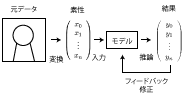
\includegraphics[width=80mm]{img/c1/ml}
 \caption{機械学習の一般的プロセス(\cite{bishop2006pattern}を基に作成)}
 \label{c1_ml}
\end{figure}
\par
機械学習の性能を上げるためには、素性への変換部分を工夫する方法と、使用する数学的モデルを洗練する方法の2つがある。素性への変換部分の改良は、対象となるデータの種類に強く依存している。例えば、画像データを素性数値に変換する場合、単純なRGB画素データをそのまま使っても良いが、SIFT特徴量\cite{lowe1999object}やSURF特徴量\cite{bay2008speeded-up}、フィッシャーベクトル\cite{perronnin2007fisher}など、より画像の特徴を捉えた特徴量を用いることが定石となっている。音声データに対しては、時間領域や周波数領域の波形をそのまま用いることもあるが、他にメル周波数ケプストラム係数などの特徴量も使われる\cite{logan2000mel-frequency}。問題とデータ種別に応じて、利用する特徴量を工夫することにより、機械学習の識別精度や実行時間などの性能が向上することが知られている。\par
従来、特徴量は画像や音声などそれぞれのデータの専門家による、謂わば職人芸によって作られていた。その後2000年代半ばに、深層学習(Deep Learning)と呼ばれる一群の手法が台頭した。深層学習とは機械学習の手法の1つで、人間の脳の構造に類似した、多層ニューラルネットワーク構造をモデルに用いて、学習を行わせる方法である。深層学習には、今まで専門家によって行われてきた特徴量の変換方法それ自体も、習得する能力があると考えられている。生のデータを入力して学習させると、データから自動的に素性を作り、抽象表現を習得することが出来るようになるのである。この深層学習は、画像認識や音声認識、化合物の生成予測といった分野で優れた性能を示し、注目を浴びるようになった。図\ref{c1_nikkei}は、多層ニューラルネットワークが人間の脳の思考回路である、神経細胞のつながりを模倣する様子を表している。\par
%注目の表現で、googleやnips2013の様子、buyoutなど
\begin{figure}[tbp]
 \begin{center}
  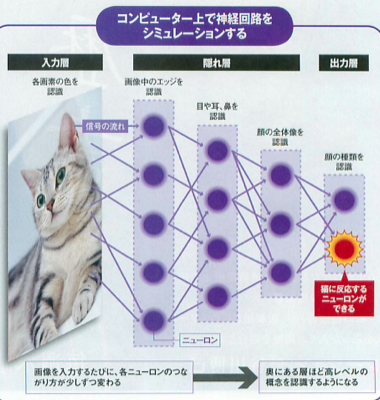
\includegraphics[width=80mm]{img/c1/nikkei}
 \end{center}
 \caption{深層学習で画像を認識する流れ (日経ビジネス2013年4月号より一部抜粋)}
 \label{c1_nikkei}
\end{figure}
深層学習の特徴の一つである、素性学習について、詳しく述べる。例えば人間の顔画像データを学習させた場合、多層ニューラルネットワークを構成する複数のレイヤーのうち、入力に近い低レイヤーのニューロンは、画像のエッジ部分に対して強く反応し、出力に近い高レイヤーのニューロンでは、目口鼻、さらに顔全体など、より抽象度の高い要素に対して反応することがわかった。これは、見方を変えれば、低レイヤーでは中間表現(素性にあたる)を抽出しており、低レイヤーで得た素性を高レイヤーに入力することにより、より高レベルな抽象的概念に対しても優れた識別精度を実現している、と考えられる。どのような素性を使えば良い結果が出るのか、素性の抽出方法自体を同時に機械学習していることから、深層学習は表現学習(Representation Learning)とも呼ばれている。\par
図\ref{c1_lee2009_faces}は、2009年、LeeらによるConvolutional Deep Belief Networkの実験によって学習された顔の要素である\cite{lee2009convolutional}。上が2レイヤー目、下が3レイヤー目で、2レイヤー目では、鼻や口、目といった顔を構成するパーツが学習されている。これは、単なる画素の数値に比べて、明らかに抽象度の高い情報に反応していると言える。さらに、3レイヤー目では人間の顔を学習することに成功している。2レイヤー目で作り出した、「顔のパーツ」という素性を元にして、さらに抽象度の高い、人間の顔という要素を推論しているのである。
\begin{figure}[tbp]
 \centering
  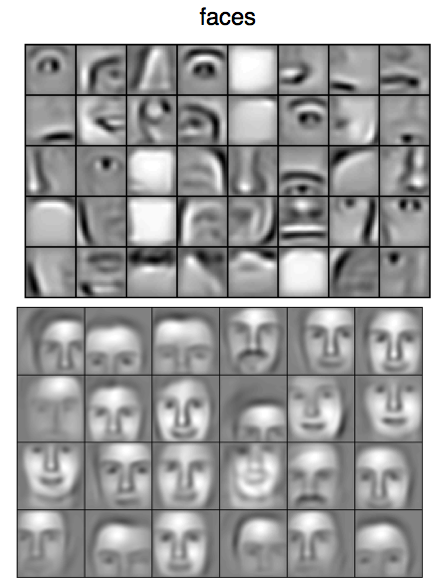
\includegraphics[width=80mm]{img/c1/lee2009_faces}
 \caption{深層学習による、顔の構成要素の学習結果(\cite{lee2009convolutional}より引用)}
 \label{c1_lee2009_faces}
\end{figure}
\par

Googleの深層学習研究グループは2012年、Youtubeのビデオから抽出した静止画による教師無し学習によって、人間や猫の顔画像を識別できる多層ニューラルネットワークモデルの学習に成功し、大きな話題を呼んだ\cite{le2012building}。\par
\begin{figure}[tbp]
 \begin{center}
  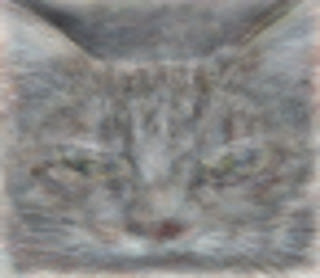
\includegraphics[width=50mm]{img/c1/cat_detection}
 \end{center}
 \caption{猫の画像に反応するニューロン (\cite{le2012building}より引用)}
 \label{c1_catdetection}
\end{figure}

\begin{figure}[tbp]
 \begin{center}
  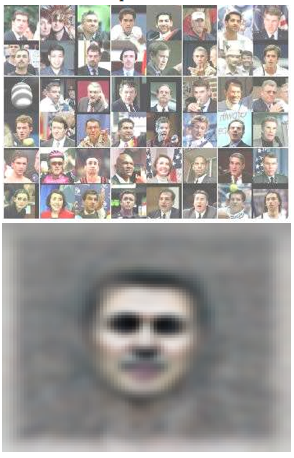
\includegraphics[width=50mm]{img/c1/google_face}
 \end{center}
 \caption{上 : 入力画像の中で、ニューロンが最も強く反応した48枚。下 : 計算上、最もニューロンが強く反応する画像\newline  (Googleの研究紹介記事より引用。http://googleblog.blogspot.jp/2012/06/using-large-scale-brain-simulations-for.html)}%
 
 \label{c1_facedetection}
\end{figure}


\section{深層学習の課題と、研究の目的}
深層学習が高い識別性能を持つことがわかり、深層学習を身近な問題に適用して、良い成果を得たいという機運が高まっている。例えば、ウェブ工学の分野では機械学習が大きな役割を果たしており、この学習プロセスに深層学習を組みこむことで、学習精度が向上したり、より多様な情報を扱えるようになる可能性がある。出来るだけ簡易に、深層学習を様々な問題に応用するための方法論が求められている。\par
しかし、深層学習は歴史の浅い発展途上の技術であり、そもそも正しい実装を行って論文同様の分類精度を発揮すること自体が難しい。また、学習時間が長く大きなマシンパワーが必要になることが多い。原理が複雑で実世界での応用例もまだ少ないため、プログラム開発に長い時間がかかってしまう。つまり、ウェブ工学など応用分野に深層学習を適用したいと考えても、実際の問題に深層学習を試行して結果を出すこと自体が困難であり、応用技術開発のハードルは更に高くなってしまっている。特に、国内での研究開発は遅れており、早急なキャッチアップが必要である。\par
本研究では、このような現状を踏まえ、深層学習技術をウェブ工学など実際の問題に応用するために、「分類精度の問題」「学習時間の問題」「実装難易度の問題」という3つの応用上の問題点に注目し、これを出来る限り緩和するための方策を提案する。\par
2章では、従来のウェブ工学における機械学習の応用方法と、深層学習出現以前に良く用いられていた、機械学習による識別器学習方法について、俯瞰する。3章では、深層学習を構成する個々のアルゴリズムについて、その原理と詳細を述べる。4章では、実際に深層学習アルゴリズムを利用する上で、どのように実装を進めれば、先に上げた問題点を緩和できるのかを述べる。5章では、深層学習のプログラムを、汎用的なベンチマークにかけることで、その性能を測定・比較する。6章では、5章までの結果を受けて、深層学習を利用していく上でのベストプラクティスを考察する。

% !TEX root = thesis.tex
\chapter{関連研究}
深層学習が登場する以前より、機械学習の技術はウェブ工学の発展に大きく貢献してきた。この章では、深層学習以前の機械学習とウェブ工学の関わりについて述べる。

\section{ウェブ工学と機械学習}
この節では、ウェブ工学における課題をいくつか例示し、それらの課題を解決するために、機械学習がどのように用いられてきたかを概観する。ただし、ウェブ工学が扱う分野は広く、その全てを述べることは難しい。そこで、ここでは特に深層学習の威力が発揮出来そうな分野として、推薦システム、リンク予測、感情分析、順位付け学習の4つを取り上げる。

\subsection{推薦システム}
主にウェブショッピングを含むサイトや、ウェブ広告の配信において求められる技術である。ウェブサイトを閲覧しているユーザに対し、そのユーザが購入したいと商品を予測して、ウェブ上の広告などの形で推薦する。適切な広告を表示することにより、ユーザの購買行動を促進することが出来る。
推薦システムの研究は、1992年のTapestryシステムに始まる\cite{goldberg1992using}。また、少なくとも90年代の終わりには、Amazon.com、CDNOW、eBay、Levis、GroupLensなど、様々なサイトにて推薦システムは利用されていた\cite{resnick1997recommender}。
推薦システムを実現するための、機械学習のテクニックとしては、大きく2種類が挙げられる\cite{koren2009matrix}。1つは、コンテンツベースのフィルタリングと呼ばれ、ユーザや商品の属性や購買傾向を学習することことで、推薦を行う。もう1つは協調フィルタリングと呼ばれており、ユーザや商品の属性を扱う代わりに、購入や評価といった、ユーザの過去の行動を基にして、推薦を行う。
%recsysなど会議
%deep learningとの関わり

\subsection{リンク予測}
リンク予測とは、図\ref{c2_link_prediction}のように、現在の時間$t$のグラフ構造(ノード間接続の様子)が与えられたとき、未来の時間$t+1$における、同じグラフの構造変化を予測する問題である。テストデータでは、グラフ中の一部のエッジが隠されており、復元の精度によって性能が測られる。\par
\begin{figure}[tbp]
 \centering
  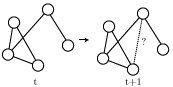
\includegraphics[width=80mm]{img/c2/link_prediction}
 \caption{リンク予測の問題設定}
 \label{c2_link_prediction}
\end{figure}
最初に提唱された論文\cite{liben2007link}では、ソーシャルネットワークの状態が与えられたとき、ユーザ間で交わされる将来の行動を予測する問題として述べられている。この論文では、ノード(ユーザ)間の近さを定義する方法や、全てのエッジ(接続)を通しで見て判断する方法、クラスタリングによる方法などが用いられている。論文で用いられているノード間の近さの定義を図\ref{c2_lp_method}に挙げる(\cite{liben2007link}より引用)。ノード$x$に対し、$x$とつながっているノードの集合を$\Gamma(x)$とする。\par
\begin{table}[tbp]
 \begin{center}
  \caption{リンク予測にて、ノード同士の近さを定義する方法}
  \begin{tabular}{|l|l|}\hline
  グラフ距離 & (負値にされた) xとyの最短距離 \\ \hline
  共通隣接 & $|\Gamma(x)∩\Gamma(y)|$ \\ \hline
  Jaccard係数 \cite{jaccard1902lois}& $\left| \frac{\Gamma(x)∩\Gamma(y)}{\Gamma(x)∪\Gamma(y)} \right|$ \\ \hline
  Adamic / Adarスコア \cite{adamic2003friends}& $\sum_{z\epsilon \Gamma(x)∩\Gamma(y)} \frac{1}{log|\Gamma(x)|}$ \\ \hline
  優先的選択 & $|\Gamma(x)|・|\Gamma(y)|$ \\ \hline
  \end{tabular}
 \end{center}
 \label{c2_lp_method}
\end{table}

リンク予測には様々な応用があり、例えばショッピングサイトのデータ分析に役立てることが出来る\cite{clauset2004finding}。ウェブ工学の問題以外にも応用が可能であり、タンパク質の反応予測(Protein to Protein Interaction, PPI)に用いられたり\cite{bader2003gaining}、テロリストのネットワークや草原の食物連鎖の分析にも役に立っている\cite{clauset2008hierarchical}。全ての部分グラフをカウントする方法はNP困難であり、計算時間的に解くことが難しいことが知られている\cite{gartner2003graph}が、この問題はGraphHopperカーネルを用いることで、現実的な時間で解くことができる\cite{feragen2013scalable}。また、Noisy ORを用いて局所的な情報を統合することにより、効率良く様々な情報を扱わせることができる\cite{changpinyo2013similarity}。
%2011のやつ、flickr, 全解析
%リンク予測の絵
%bag of words?

\subsection{感情分析}
この場合の感情とは、人間が書いた文章から読み取れる感情を指す。ウェブ上の情報収集の自由度が高まるにつれて、ユーザが書いた文章を取得できる機会が増えてきている。その中には、新製品やサービスへの感想やレビューも含まれている。ユーザの属性や行動といった明確な事実だけでなく、他の人がどのような感情を抱いているのかを分析したいという要望が高まり、2000年代に入ってから、人間が書いた文章から人間の感情を読み取るための研究が盛んになった\cite{pang2008opinion}。なお、意見抽出(opinion mining)という語も、多少の差異はあれど、広義には似た内容を指していることが多い。\par
\cite{pang2004sentimental}では、最小カット法を用いることで良い成果が出たとされている。また、\cite{wilson2005recognizing}では、文脈を考慮した単語の感情(positive, negative)を分析して、性能を挙げることに成功している。Google社も、検索エンジンの性能向上のため、感情分析の研究を行っている\cite{godbole2007large}。\par
深層学習との関連で重要な研究として、Stanford大のチームによる文章解析データセットの制作及び、ウェブアプリの開発がある\cite{socher2013recursive}。この研究にて彼らは、感情分析のための大規模なデータセットがそもそも不足しているという問題を解決するため、The Stanford Sentiment Treebankという感情分析のためのデータセットを制作した。さらに、Recursive Neural Tensor Network (RNTN)という深層学習のモデルを構築した。このモデルにより、与えられた文章を構文木に分解した後、各単語が5段階の感情のうちどれにあたるかを分析している。感情は、"very negative"、"negative"、"neutral"、"positive"、"very positive"の5種類に分類される。このモデルは、ソースコードが公開されている他、ウェブページ上にて実際に分析を試してみることができる\footnote{\url{http://nlp.stanford.edu/sentiment/index.html}}。図\ref{c2_rntn_ex}は、論文より引用したもので、文章を実際にこのウェブアプリで分析した様子を表している。赤が強いと悲観的(negative)な言葉、青が強いと好意的(positive)な言葉、というように色分けされている。
\begin{figure}[tbp]
 \centering
  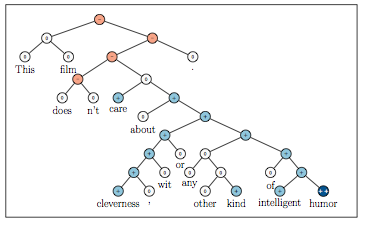
\includegraphics[width=80mm]{img/c2/rntn_ex}
 \caption{Stanford大が製作した、深層学習による感情分析の例}
 \label{c2_rntn_ex}
\end{figure}

\subsection{順位付け学習}
これは、情報検索システムを作る際に用いられる技術である。ユーザが検索をかけるときは、自分が求めた情報だけを、出来るだけ取りこぼし少なく取得したい(適合率と再現率という。\cite{tsujii1999joho})。従来はtf-idfやPageRank\cite{brin1998anatomy}\cite{page1999pagerank}などの単一の指標によって、検索結果を表示させていたが、その後多様なランキング素因を組み合わせるという方法が出現した。どの素因をどのような割合で組み合わせるべきかが問題であり、これに対し機械学習によってランキング関数を作成するアプローチが、順位付け学習である。\par
RankNet\cite{burges2005learning}では、深層構造こそ使っていないが、ニューラルネットワークによってランキング関数の性能をアップさせており、深層学習の応用による性能向上が期待できる。

\section{機械学習で利用される、代表的な分類器}
機械学習のプロセスは、「入力データを、数学的モデルで使える素性に変換する」「素性を数学的モデルに入力して、出力値を得る」「出力を見ながら、モデルを修正する」という行程に大きく分けられる。データの分類問題を機械学習で解く場合、モデルによる出力値が分類結果に対応するよう、モデルを学習させることになる。この場合、モデルのことを分類器とも呼ぶ。\par
機械学習において、素性への変換部分は、データの種類に大きく依存する。一方、分類器に用いる数学的モデルと、モデルの改修法、つまり学習法は、汎用的に使うことができる。あるいは、画像や音声、文章といったデータの多様性を、素性という一般的な数値に落とし込むことで吸収して、汎用的分類モデルでも学習できるようにしている。\par
深層学習、あるいは深層ニューラルネットワーク(多層ニューラルネットワーク)は、汎用的分類モデルの一種である。ここでは、深層学習の他にどのような分類器が存在するのか、代表的なものを述べる。
%\subsection{線形識別モデル}

%\subsection{ロジスティック回帰}
%random forest, ada boost

\subsection{サポートベクターマシン}
サポートベクターマシン(SVM)は、図\ref{c2_svm}のように、データを2つのクラスに分類する能力を持ったモデルである\cite{cortes1995support-vector}。\par
SVMのメインとなる原理は、マージン最大化である。図\ref{c2_svm}は最も単純なSVMの問題を表しており、グラフ上に散らばった黒と白の点を、直線を1本引くことで分けることが目標である。言い換えれば、どの点が黒で、どの点が白なのかを識別する、2クラス分類問題を解こうとしている。緑の線は、分類に失敗している。青の線は分類に成功しているが、後から点線で表された新しい白点が加わると、やはり分類に失敗してしまう。赤の線は、現在見えている点を分類できるだけでなく、新しい点が加わっても正しく識別できる可能性が高い。SVMのマージン最大化とは、各点からの距離(マージン)の和が、最大になるように直線の引き方を決めることである。こうすることにより、汎化性能(訓練時に見えていなかった、新しいデータを正しく分類する性能)が最大になることが知られている。\par
この図のSVMは、データが直線で完全に分類できることを前提にしている。しかし、現実のデータは、\ref{c2_svm_mixed}のように、必ずしも1本の直線にて分類が可能ではない。(3次元以上の場合で言えば、1つの超平面にて分類が可能とは限らない。)このような場合に対応するため、まず非線形関数にてデータを高次元の空間に移し、超平面による分類が出来るように変換する方法が知られている\cite{burges1998tutorial}。ただし、一般に複雑な分類ほど、変換先の次元数が高くなる傾向があり、次元数が増えると、「次元の呪い」と言って、内積計算にかかる時間が指数関数的に増大することがわかっている\cite{bellman1961adaptive}。この計算時間を減少させるため、数式処理によって内積を計算する必要がなくなるように設計された、カーネル関数と呼ばれる変換関数を用いる方法が使われている(カーネルマジック)。
\begin{figure}[tbp]
 \centering
  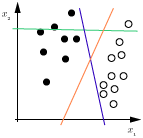
\includegraphics[width=80mm]{img/c2/svm}
 \caption{サポートベクターマシンのマージン最大化}
 \label{c2_svm}
\end{figure}
\begin{figure}[tbp]
 \centering
  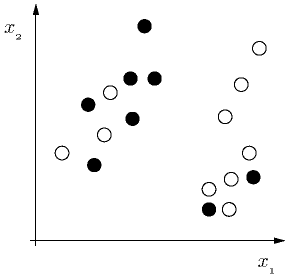
\includegraphics[width=80mm]{img/c2/svm_mixed}
 \caption{直線にて分類できない場合}
 \label{c2_svm_mixed}
\end{figure}
SVMは、広くその信頼性が認められたモデルの1つであり、ライブラリの利用方法も確立している。例えば、LIBSVM\footnote{\url{http://www.csie.ntu.edu.tw/~cjlin/LIBSVM/}}やLIBLINEAR\footnote{\url{http://www.csie.ntu.edu.tw/~cjlin/LIBLINEAR/}}は使用が容易なライブラリとしてよく知られている。これらのライブラリを使うと、簡単な所定の方式に沿って入力データファイルを用意し、CUI上で2,3回の操作をするだけで、SVMによる分類を行わせることができる。このとき、利用者が自分でプログラムを書く必要は全くない。プログラムを書かないで済むと、手軽に利用することができ、またバグを起こす危険性が非常に少なく安全に使うことができる。\par
深層学習については、このようなライブラリはまだ存在していないため、深層学習の代表的なアルゴリズムについて、プログラム無しで利用できるようなライブラリの整備が望まれる。
\subsection{ニューラルネットワーク}
ニューラルネットワークは、人間の脳の構造を模倣した数学的モデルである。人間の脳は、ニューロンと呼ばれる神経細胞が大量に接続されて出来ている。ニューロンが電気信号を伝達することで、様々な脳の働きが行われている、と考えられている。プログラム上で表現されるニューラルネットワークには、人間の脳の動作との相違点もあり、脳が行っている計算を正しくシミュレートしているとは言い難い面もある\cite{kawato1998}が、機械学習のモデルとしては広く使われてきた。\par
\subsubsection{ニューラルネットワークの伝達方式}
以後、機械学習におけるニューラルネットワークのニューロンを、慣例に従ってユニットと呼ぶことにする。ニューラルネットワークでは、ユニットからユニットへの接続が網目のように広がっている。ユニットは入出力の機能を持つ。これは、生体におけるニューロンが、他のニューロンから化学的な刺激を受け取り、受け取った刺激に応じて自らも他のニューロンを刺激する構造を真似ている。ユニットは入力を受け取ると、活性化関数(activation function)を使って入力値を変換し、接続先のユニットへ出力する。このとき、ユニットからユニットへの結線に、重み(weight)と呼ばれる係数を付与して、出力を変化させることが普通である。これは、生体のニューロン同士の接続が、脳の学習につれて強固になり、刺激がより伝わりやすくなっていくことに対応させている。
\subsubsection{パーセプトロン}
パーセプトロン(perceptron)とは、ニューラルネットワークの一種である。複数のユニットをまとめたレイヤーが、いくつか重なって出来ており、値の伝達は入力レイヤーから出力レイヤーへの一方向に限られているものを指す(前送り)。狭義には、単層かつ活性化関数にヘビサイド関数を用いた2クラス分類モデルのみを指すこともある。\par
始めに提唱されたのも、入力層と出力層の2層から成る、単層パーセプトロンと呼ばれるモデルだった\cite{rosenblatt1958perceptron}。このモデルは、後に線形関数しか近似できないことがわかり、いったん下火になった\cite{minsky1988perceptrons:}。例えば、単層パーセプトロンでは、非線形関数であるXOR関数を学習させることが出来なかった。\par
しかし、隠れ層を追加し、活性化関数にシグモイド関数などの非線形関数を用い、さらにバックプロパゲーションという方法で学習を行わせることにより、非線形関数を近似可能となることがわかり、再び有用な識別モデルとして脚光を浴びた\cite{rumelhart1986learning}\cite{funahashi1989on-the-approximate}。これを単層パーセプトロンと区別して、多層パーセプトロン(Multi Layer Perceptron, 以下MLP)とも呼ぶ。このモデルは単純な2クラス分類モデルの範囲を逸脱しており、元々のパーセプトロンとはやや異なるものだが、慣例的にこのように呼ばれている。\par
バックプロパゲーションは教師有り学習の一種である。出力層におけるモデルが出した推定値と、教師データの結果が異なっている場合、教師データからの推定誤差(error)が減少するように、モデルのパラメータを修正する。MLPの場合、モデルのパラメータとはユニット間の伝達にかかる重み係数のことである。パラメータの修正値の仕方にはバリエーションがあるが、最もよく使われるのは確率的勾配降下法(以下SGD)と呼ばれる方法である。これは確率変数に拡張された一種の再急降下法である。直感的に言えば、微分によって、その場で推定誤差が最も急速に減少するパラメータの修正方向を算出し、その方向に向かってパラメータを変化させる。SGDを少し変化させ、複数のデータによる誤差を一度に処理するバッチ勾配降下法(BGD)や、SGDの1次精度に対し、2次精度までの情報を使う共役勾配法(Conjugate Gradient Method, CG)も存在する。\par
%vanishing error problem
バックプロパゲーションを行うためには、活性化関数が微分できることが重要である。シグモイド関数は、元々使われていたヘビサイド関数に形が似ている上に、微分が容易という点でバックプロパゲーションとの親和性が高く、有利である。しかし、シグモイド関数のデメリットとして、入力と重みの積が大きくなるにつれて、誤差への反応が小さくなってしまい、学習の進行が遅くなるという問題を抱えていた。この問題は、特にバックプロパゲーションで伝播する距離が長くなる構造にて顕著になった\cite{hochreiter1998the-vanishing}\cite{hochreiter1998the-vanishing}。このため、多層ニューラルネットワークを学習させる方法は長い間課題となっていた。
% !TEX root = thesis.tex
\chapter{深層学習の成果とアルゴリズム}
深層学習は、多層ニューラルネットワーク(MLP)のうち、普通隠れ層が2つ以上のものをいう。2006年にHintonらによって、このようなDeepな構造を学習させる方法が発見され、発展への道が開けた\cite{hinton2006a-fast, hinton2006reducing}。従来よりも多くのレイヤーを扱うことで、より複雑な関数を学習できるようになった。深層学習は、数々の分類タスクにて、従来手法を大きくしのぐ成果を収め、注目を浴びている。この章では、深層学習で使われているアルゴリズムの詳細について述べる。
\section{深層学習の成果}
第1章でも触れたが、2012年には、GoogleがSupervisionと題してYoutubeビデオの静止画を使って多層ニューラルネットワークの教師なし学習を行わせ、結果として、猫を認識するユニットや人を認識するユニットを学習させることに成功した。また、ImageNet Large Scale Visual Recognition Competition(ILSVRC)というデータセット\cite{deng2009imagenet:}の分類にて、最先端の結果を残した。ImageNet\footnote{\url{http://www.image-net.org/}}とは、WordNet\footnote{\url{http://wordnet.princeton.edu/}}を真似して作られたデータセットである。2009年より、100を超える様々な論文にて、画像認識のベンチマークに利用されてきている\footnote{\url{http://www.image-net.org/about-publication}}。図\ref{c3_imagenet}は、ImageNetの画像の例である。画像はツリー状に分類されており、例えば上を見ると、mammal(哺乳類)→palcental(胎盤)→carnivore(肉食)→canine(イヌ科)→dog(イヌ)→working dog(盲導犬やそり犬など使役される犬)→husky(ハスキー)というように、徐々に分類が細かくなっていくことがわかる。また、一つのカテゴリーには、9枚の画像がひもづけられている。\par
\begin{figure}[tbp]
 \begin{center}
  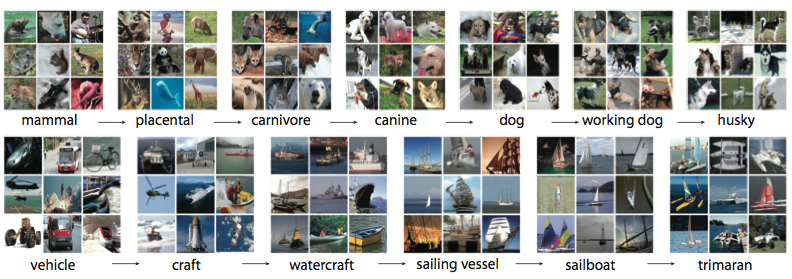
\includegraphics[width=120mm]{img/c3/imagenet}
 \end{center}
 \caption{Imagenetの画像とラベル構造の例}
 \label{c3_imagenet}
\end{figure}
Googleのsupervisionによる、画像分析の結果の例を図\ref{c3_supervision}に載せる(\cite{krizhevsky2012imagenet}より引用)。画像の分類に失敗している場合でも、妥当なラベルをつけていることがわかる。\begin{figure}[tbp]
 \begin{center}
  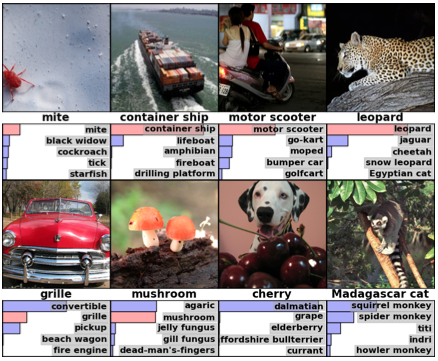
\includegraphics[width=80mm]{img/c3/supervision}
 \end{center}
 \caption{Supervisionによる画像分類の結果の例}
 \label{c3_supervision}
\end{figure}

深層学習は画像分析だけでなく、自然言語処理(NLP)の分野でも有効なことがわかっている。Googleが公開している"word2vec"というライブラリを使うと、入力されたテキスト文書から、単語のベクトル化やクラスタリングを行うことができる\cite{mikolov2013efficient}\cite{mikolov2013linguistic}。このベクトル化により、
\begin{equation}
vector('Paris') - vector('France') + vector('Italy') = vector('Rome')
vector('king') - vector('man') + vector('woman') = vector('queen')
\end{equation}
のような計算が行えるようになった。また、この計算を行う過程で、全ての単語同士の内積の和を計算していたところを止め、数個だけサンプルを取って計算することで、計算時間が短縮できるだけでなく、分類精度まで向上することが判明した\cite{mikolov2013distributed}。\par
word2vecを応用した研究も出現している。Deep Visual-Semantic Embedding model(DeViSE)\cite{frome2013devise}と名付けられたシステムでは、zero-shot learningと呼ばれる問題を解かせるため、Supervisionとword2vecを組み合わせている。zero-shot learningとは、訓練時に一度も見たことがないクラスの画像に対し、正しく分類を行えるかという問題である。この研究では、1000カテゴリの画像による訓練を行っただけで、まだ見たことが無い20000カテゴリに属する画像を適切にラベリングしている。画像以外に全く情報がなければ分類は不可能なので、wikipediaのテキスト内容を補助データとして使っているが、これはWordNetや意味データベースの情報を直接用いていた従来の研究\cite{mensink2012metric}\cite{rohrbach2011evaluating}\cite{palatucci2009zero-shot}に比べて、より生データに近い情報で処理に成功していると言える。\par
\begin{figure}[tbp]
 \centering
  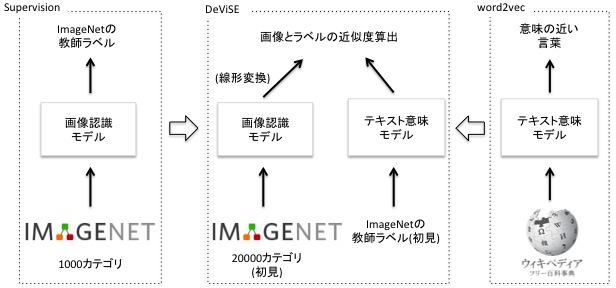
\includegraphics[width=120mm]{img/c3/devise}
 \caption{DeViSEの学習方法}
 \label{c3_devise}
\end{figure}
図\ref{c3_devise}は、DeViSEの学習方法を示している(ImageNetとWikiediaのロゴは、公式ウェブページより引用した\footnote{\url{http://www.image-net.org/splash/logo.jpg}},\footnote{\url{http://upload.wikimedia.org/wikipedia/commons/a/ad/Wikipedia-logo-v2-ja.png}})。DeViseでは、画像データを意味付けするためにSupervisionを使い、wikipediaの情報処理にword2vecを用いている。まずSupervisionにImageNetのデータを、word2vecにwikipediaのデータを与えて学習させたあと、実際の画像及び未見カテゴリのラベルを与え、画像とラベルの意味ベクトルが、出来るだけ近くなるように分類している。\par
深層学習を強化学習(reinforced learning)と組み合わせることで、ゲームを上手くプレイできるAIを作る研究も成功している\cite{mnih2013playing}。強化学習では、環境に対してAIが行動を起こし、環境から得られる報酬を最大化できるように、アルゴリズムを修正していく。多くの場合、「行動と報酬の間に時間差があり、どの行動が報酬に結びついたのか分かりにくい」「行動によって環境が変化しててしまうため、分析が難しい」といった状況設定がなされる。また、Bandit問題というカテゴリでは、スロットゲームを題材にして、「知識を活用すると報酬は上がるが、もっと良い行動があるかもしれない」「行動の探索を優先すると、既存知識は活かせず、一時的な報酬は下がりやすい」というジレンマの解決が研究されている\cite{cesa-bianchi2013a-gang}。\cite{mnih2013playing}の研究では、ゲーム内のキャラクターをAIで行動させ、報酬としてのスコアを最大化させるような行動を学習させる。深層学習は、ゲーム内の状況をモデル化して、そこから最適な行動を導き出すために用いられている。

\section{深層学習のアルゴリズム}
\subsection{深層信念ネットワークwork}
最初にMLPの学習のブレイクスルーとなったのは、2006年のHintonらによる深層信念ネットワークs(DBN)\cite{hinton2006a-fast, hinton2006reducing}である。このモデルについて解説する。
\subsubsection{教師無し 事前学習と微調整}
この研究では、MLPの重みをランダムに初期化した後、すぐバックプロパゲーション学習にかけるのではなく、各レイヤーの重みをあらかじめ教師無し(教師無し)学習で調整して、隠れ層が効率の良い素性を学習できるよう仕込んでおくというアイデアが使われた。この事前学習のことを、事前学習と呼び、バックプロパゲーションにて学習する段階の方は、微調整と呼ぶ。事前学習の段階では、入力側から1レイヤーずつ学習を行い、学習済のレイヤーは固定して動かさない(Greedy レイヤー-wise 事前学習)。微調整の段階では、全てのレイヤーをバックプロパゲーションにて同時に変化させていく。DBNの構造を、図\ref{c3_dbn}に示す。\par
\begin{figure}[tbp]
 \centering
  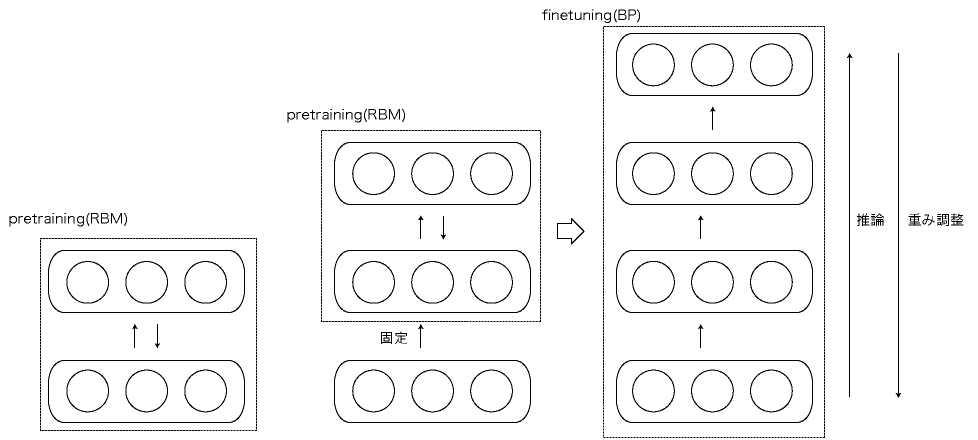
\includegraphics[width=120mm]{img/c3/dbn}
 \caption{深層信念ネットワークworkの構造と、学習過程}
 \label{c3_dbn}
\end{figure}
教師無し 事前学習をどのような基準で行うかが問題だが、この研究では、制限付きボルツマンマシン(以下RBM)というモデルを用いている。RBMとは、ニューラルネットワークの一種で、可視変数層と隠れ変数層の2つのレイヤーから成り立っている。DBNにおいては、可視変数=入力データと考えておけばよい。RBMモデルの学習を進めることで、入力データ→隠れ変数への推論モデルを得ることができる。これが深層学習の最大の特徴の1つである、「抽象度の高い素性への変換方法自体を学習する」ことに対応している。DBNでは、RBMを1レイヤーずつ学習させながら、RBM同士を「前のレイヤーの隠れ層 = 次のレイヤーの入力層」となるようにつなげていく。これにより「入力層→抽象度の低いレイヤー→...→抽象度の高いレイヤー→出力」という、複数の隠れ層をもつDeepな構造を作り、上手く事前学習させることに成功している。RBMを積み重ねた最も上のレイヤーに、普通の線形レイヤーを1つ置いて、「最も抽象度の高い素性→出力値」の推測を行わせることが多い。なお、微調整におけるバックプロパゲーションでは、RBMにあった「隠れ層→入力層」の方のつながりは、最終レイヤーにおける誤差に影響しない。よって、以前からある前送りなMLPと同様に学習させることができる。
\subsubsection{制限付きボルツマンマシン}
DBNの事前学習に用いられる制限付きボルツマンマシン\cite{smolensky1986information}とは、ニューラルネットワークを用いた生成モデルの一種である。まず生成モデルについて説明する。\par
クラス分類問題を確率的アプローチで解く方法は、生成モデル(generative model)と識別モデル(判別モデル、discriminative model)の2つに大別できる\cite{bishop2006pattern}\footnote{確率モデルを介さず、入力からクラスを得る識別関数を直接導くことも出来る。}。クラス分類問題では、まずクラス事後確率$p(C_k|x)$を各クラス$k$に対して求める。基本的には入力$x$に対して最もクラス事後確率が大きくなったクラスに分類することになる\footnote{医療における誤診断など、誤分類のタイプに応じて重要度が異なる場合、損失関数(loss function)を導入することもある。}。識別モデルでは、クラス事後確率$p(C_k|x)$のみを直接学習するのに対し、生成モデルでは、まずクラスの条件付き密度$p(x|C_k)$を学習する。これと、別途求めたクラスの事前確率$p(C_k)$を用いることで、クラス事後確率は
\begin{equation}
p(C_k|x) = \frac{p(x | C_k)p(C_k)}{p(x)} = \frac{p(x | C_k)p(C_k)}{\sum_{k}p(x | C_k)p(C_k)}
\end{equation}
によって求められる。これは、入力とクラスの同時確率$p(C_k, x)$を求めることと等価である。生成モデルの利点は、クラス分類のモデルだけでなく、入力データの性質に関する情報をも同時に得られる点にある。しかし、一般に識別モデルよりも複雑で困難な問題を解く必要が生じるため、常に生成モデルが用いられるわけではない。\par
\begin{figure}[tbp]
 \centering
  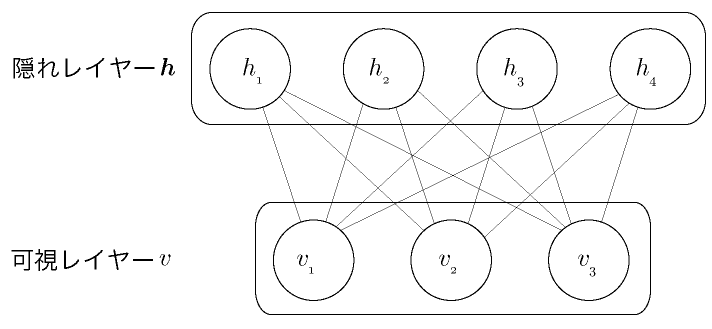
\includegraphics[width=100mm]{img/c3/rbm}
 \caption{Restriceted Boltzman Machineのネットワーク構造}
 \label{c3_rbm}
\end{figure}
さて、前述したように、RBMは可視層と隠れ層の2レイヤーで構成されるニューラルネットワークである。RBMの構造を、図\ref{c3_rbm}に示す。入力層の各ユニットの値を$v_j$, 隠れ層の各ユニットの値を$h_i$とおく。これらをまとめたベクトルをそれぞれ$\bm{v}=\{v_1, v_2, ...\}, \bm{h}=\{h_1, h_2, ...\}$とおく。これは、例えば$\bm{v}$が画像や音声などの入力データをベクトル化したもので、$\bm{h}$がこれらの変数の関係を説明する変数だと考えれば良い。ただし、$\bm{h}$が即$\bm{v}$のクラス分類に対応するとは限らないことに注意する。RBMの学習を進めると、$p(\bm{v}|\bm{h})$と$p(\bm{h}|\bm{v})$との、2方向の条件付き確率のモデルが同時に得られる。\par
RBMの学習は、自由エネルギーと呼ばれる従属変数を最小にするように行われる\footnote{自由エネルギーという呼び名は、物理学から採られている。}。ここでは、最も簡単かつ重要な、$v_j, h_i\epsilon\{0,1\}$のケースについて述べる。Wをvとhの間の重み、bとcを、それぞれvとhに対応するバイアス項とする。このとき、RBMにおける自由エネルギー$F(v)$は、
\begin{equation}
F(v) = -b' v-\sum_{i}log(1+e^{(c_i+W_{i}v)})
\end{equation}
となる。この自由エネルギーを、SGDなどのアルゴリズムを用いて最小化することで、目標となる生成モデルを得ることができる。なお、自由エネルギーの導入と最小化というアプローチは、エネルギーに基づくモデルと呼ばれるアルゴリズム群に共通して用いられる概念であり、自由エネルギーにもさらに様々なモデルで使える一般的な定義が存在するが、割愛する。
\subsubsection{DBNの性能}
この研究では、評価実験としてMNISTの手書き数字認識データセットを用いている。彼らは各レイヤーのユニット数が"784-500-500-2000-10"という構造のDBNによって、学習を行った。そして、順序不変と呼ばれるタスクにて、当時のstate fo the artを塗り替えたことにより、注目された。ここで、順序不変とは、データを単なる1次元の値の集まりと見なし、2次元の画像という事前情報の利用を禁止した状態で、分類実験を行うことである。具体的には、画像的変形による水増しや、2次元的畳み込み(畳み込みレイヤーの節にて詳述)などが当てはまる。順序不変の制約下で良い成果を出したDBNは、画像の性質を利用した畳み込みネットワークに比べたとき、画像以外の1次元のデータに対しても適用しやすいアルゴリズムだと考えられる。

\subsection{積層雑音除去自己符号器}
深層信念ネットワークworkと共に、1次元のデータに対して広く用いることができるモデルが、積層雑音除去自己符号器である。これは2007年に提唱されたStacked 自己符号器\cite{bengio2007greedy}というモデルを基に、2008年に発表された\cite{VincentPLarochelleH2008}。基本的なアイデアは、深層信念ネットワークsにおけるRBMを、雑音除去自己符号器というモデルに変更することである。
\subsubsection{自己符号器}
雑音除去自己符号器は、自己符号器の特殊なバージョンなので、まずは自己符号器について説明する。自己符号器は、ニューラルネットワークの一種であり、入力されたデータを再現するようなモデルを学習する。\cite{bourlard1988auto, hinton1994autoencoders, schwenk1995transformation}\par
自己符号器の構造を、\ref{c3_自己符号器}に示す。自己符号器は、この図でいうInput, Representation, Outputの3つのレイヤーから構成されている。OutputとInputの値が一致するように、重み$W$と$W'$を学習させていく。この一致に成功すれば、RepresentationはInputを復元(decode)するための情報を含んでいる、つまりRepresentationはInputの別表現である、という論理が成り立つ。Inputに与えられたデータを、別の素性を用いたRepresentationに符号化(encode)していることから、自分自身の符号化方法を覚えるという意味で、自己符号器という名前がつけられている。\par
自己符号器を用いることで、Inputを別の素性に変換することができる。しかし一方で、必ずしも得られた素性が抽象度の高いものになっているとは限らない。例えば、最も自明な自己符号器は、EncoderとDecoderの双方に恒等写像を用いることである。このとき、InputとRepresentationとOutputの値は一致し、確かにReconstruction Errorは0になっている。しかし、InputとRepresentationの抽象度は同じであり、素性学習としての有用性は全くない。実用上は、SGDを用い、入力レイヤーよりも表現レイヤーのユニット数を多くとり、非線形な関数をEncoderやDecoderに使うことで、抽象度が高くスパースな素性が獲得されることがわかっている\cite{bengio2007greedy}\cite{lee2007sparse}。しかし、理論的な理由は解明されていない。この素性学習の不確実性の問題を緩和するのが、次に述べる雑音除去自己符号器である。
\begin{figure}[tbp]
 \begin{center}
  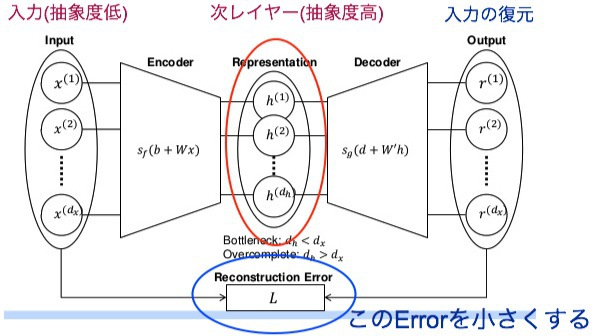
\includegraphics[width=80mm]{img/c3/autoencoder}
 \end{center}
 \caption{自己符号器の構造図}
 \label{c3_自己符号器}
\end{figure}

\subsubsection{雑音除去自己符号器}
雑音除去自己符号器は、自己符号器を拡張したものである。Input層に渡す入力データの一部をランダムに隠し(corrupted input)、元の隠されていない入力データを復元するように学習させる。データを隠す割合をcorruption rateといい、例えばcorruption rate30\%の場合、100次元の画像データだとしたら、そのうち30次元分をランダムに選んで、数値を0にしてしまうことになる。図\ref{c3_da_pic}は、雑音除去自己符号器が働く様子を、画像の入力レイヤーの場合について表している。\par
また、図\ref{c3_da}は、元の入力データ群から外れた入力データを作り、これを復元している様子を模式的に表している(\footnote{\url{http://www.iro.umontreal.ca/~bengioy/talks/icml2012-YB-tutorial.pdf}}より引用)。データの一部を隠すことによって、より頑堅な素性の作り方のモデルを得ることが出来ると考えられている。\par
なお、雑音除去自己符号器の学習過程には、制限付きボルツマンマシンのようなエネルギーに基づくモデルとの類似性があることがわかっている\cite{vincent2011a-connection}。
\begin{figure}[tbp]
 \begin{center}
  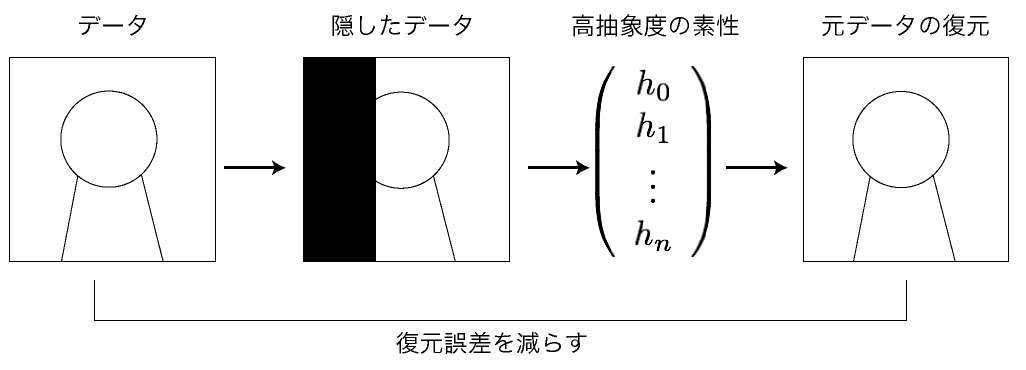
\includegraphics[width=80mm]{img/c3/da_pic}
 \end{center}
 \caption{画像に対する雑音除去自己符号器}
 \label{c3_da_pic}
\end{figure}

\begin{figure}[tbp]
 \begin{center}
  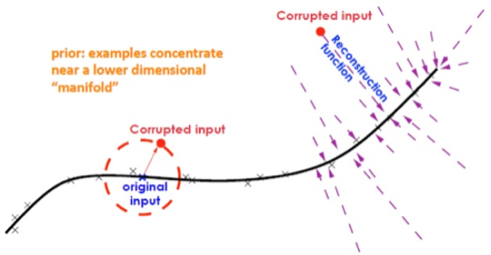
\includegraphics[width=80mm]{img/c3/da}
 \end{center}
 \caption{雑音除去自己符号器の模式図}
 \label{c3_da}
\end{figure}

\subsubsection{積層雑音除去自己符号器}
積層雑音除去自己符号器(SDA)は、深層信念ネットワークsの事前学習で、RBMの代わりに雑音除去自己符号器(以下DA)を用いたものである。DBN同様、前の層のRepresentationレイヤー = 次の層のInputレイヤーとなるように、DAで学習したレイヤーを積み重ねていく。最終レイヤーには、DAではなくソフトマックスレイヤーなどを置き、最終的な確率を出して、分類を行わせる。図\ref{c3_sda}は、SDAにて、どのように事前学習が繰り返され、DAが積み上げられていくのかを表している。いったん事前学習が済んだら、そのレイヤーの入力は隠さず、学習された重みをそのまま使って高い抽象度の素性を作る。そして、その新しい素性を入力と捉えて、新たに雑音除去自己符号器の学習を行わせる。これを繰り返してレイヤーを積み上げ、最終的に良い素性を学習しやすいMLPを作ることで、微調整段階でも学習がスムーズに進み、精度のよい推論ができるようになる。
\begin{figure}[tbp]
 \centering
  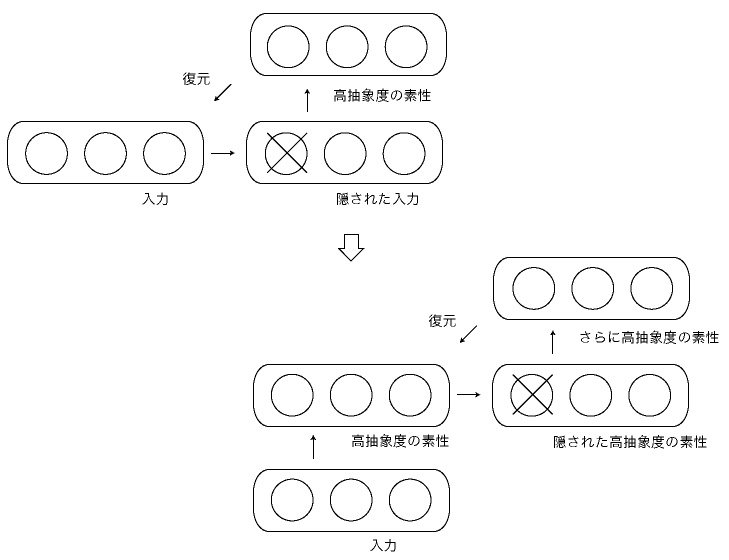
\includegraphics[width=100mm]{img/c3/sda}
 \caption{積層雑音除去自己符号器における学習の進行}
 \label{c3_sda}
\end{figure}

%深層学習の登場 Hinton, Bengio, LeCun
%画像認識タスクでの成績、音声認識タスクでの成果、猫認識
%MNIST, CIFAR, SVHNなどにおけるconv.net、Maxout, DropConnectの優位

\subsection{畳み込みネットワーク}
畳み込みネットワーク(畳み込みネットワーク)は、画像認識にて使われるニューラルネットワークの一種である。DBNやSDAのようにユニットが1対1で接続されるのではなく、画像上で距離が近いユニットを一まとめに考えるが特徴である。具体的には、フィルターと呼ばれる小さな四角形を、画像の上で動かしていき、フィルターが覆っている部分の性質を抽出して次のレイヤーに渡していく。フィルターは行列で表現されており、フィルター行列の各要素と、画像の各画素を掛け算し、その和を取ることで、次のレイヤーに渡す値が得られる。基本的な構造は、図\ref{c3_convolution}のようになっている。この図では、2回のconvolutionを行ったあと、十分に画像の素性が得られたところで、従来のMLPで見られる隠れレイヤーを1つ介して、出力を得ている。\par
\begin{figure}[tbp]
 \centering
  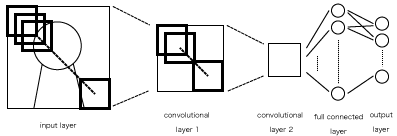
\includegraphics[width=80mm]{img/c3/convolution}
 \caption{畳み込みネットワークの仕組み}
 \label{c3_convolution}
\end{figure}
畳み込みネットワークの発祥はDBNやSDAよりも古い。画像上の各部分ごとに性質を抜き出しニューラルネットワークを構成するというアイデアは、人間の視覚野の仕組みを参考にしたもので、1980年のNeocognitronを始めとして\cite{fukushima1980neocognitron}\cite{fukushima1983neocognitron}様々な形で提唱されている\cite{lecun1998gradient-based}\cite{serre2007robust}。2003年に提唱された畳み込みネットワークのモデルが、画像認識ベンチマークのMNISTにて、今でも5位の精度を保っており\cite{simard2003best}、2012年のものは2位となっている\cite{ciresan2012multi-column}。Fisherベクトルなど既存の画像認識手法との組み合わせでも、良い性能を発揮できることがわかっている\cite{nakayama2013efficient}。ここで紹介するのは、1998年にLeCunらが紹介した方法\cite{lecun1998gradient-based}であり、ほとんどの畳み込みネットワークに使われているアルゴリズムの基本的な部分である。
\subsubsection{素性写像}
実際の畳み込みネットワークでは、素性写像と呼ばれる方法が使われている。これは、フィルタが1つだけでなく、複数種類のフィルタを、複数枚の画像の上で動かしていく方法である。図\ref{c3_convolution}の構造に、素性写像の考え方を適用すると、\ref{c3_feature_map}のようになる。この図では、フィルターが移動する様子は省略している。四角形は素性写像1つを、円はMLPのユニット1つを表している。素性写像同士では、フィルタによる畳み込みによって情報が伝達される。素性写像からMLPの隠れレイヤーにつながる部分では、まず全ての素性写像をつなげ、1次元のベクトルに並び替えて入力したと考えている。残りは、通常のMLPと同じように処理される。(なお、図\ref{c3_convolution}では、簡単のため、素性写像は表現されていない。)\par
1枚のmapが、1書類のフィルタに対応しているので、フィルタの数と同じだけ次のレイヤーの素性写像が用意されている。それぞれのフィルタを、全ての素性写像の上で動かして、畳み込み計算を行っていく。最終的に、普通のMLPに帰着させるところは変わらない。\par
素性写像は、カラー画像を扱うときにも利用できる。カラー画像データは、ほとんどの場合Red、Green、Blueの光の3原色に対応する3つの値にて表現される。これを省略してRGBと呼ぶ。畳み込みネットワークの入力レイヤーにて、画像サイズと同じ大きさの、RGBの3色に対応する3つの素性写像を設定することで、色情報を簡単に扱うことができる。

\begin{figure}[tbp]
 \centering
  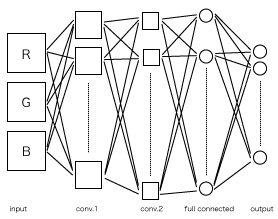
\includegraphics[width=80mm]{img/c3/feature_map}
 \caption{畳み込みネットワークと素性写像}
 \label{c3_feature_map}
\end{figure}

\subsubsection{最大値蓄積}
Convolutinal Netにて、もう1つ広く使われている方法が、最大値蓄積である。最大値蓄積レイヤーは普通畳み込みレイヤー同士の間に置かれる。最大値蓄積では、畳み込みレイヤーで得られた画素を、部分ごとにたたみ込んでいく。ただし、畳み込みレイヤーの計算に使うフィルタとは違い、重み行列は用いず、単純に対象領域の画素値のmaxを取って、次のレイヤーに渡していく。また、畳み込みレイヤーではフィルタを1ピクセルずつ動かしていくが、最大値蓄積レイヤーでは、一度にフィルタのサイズと同じだけ動かし、畳み込み対象領域が重ならないようにする。また、フィルタのサイズは2x2ピクセルに設定されることが多い。図\ref{c3_maxpooling}の左側は、最大値蓄積による畳み込みの様子を、右側では最大値蓄積 レイヤーによる畳み込みの全体の様子を表している。\par
最大値蓄積を用いることにより、各レイヤーの次元数を効率良く下げることが出来る。また同時に、ピクセルの位置が少し変化しても同じ結果が得られるので、位置的な頑健性を上げることも出来る。\par
最大値蓄積レイヤーを併用した場合の、一般的な畳み込みネットワークの全体図を、図\ref{c3_convnet}に挙げる。なお、この図では、各素性写像ごとのつながりは省略している。

\begin{figure}[tbp]
 \centering
  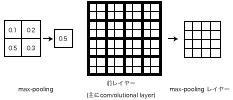
\includegraphics[width=80mm]{img/c3/maxpooling}
 \caption{Maxpoolingと、Maxpooling レイヤーの作用}
 \label{c3_maxpooling}
\end{figure}

\begin{figure}[tbp]
 \centering
  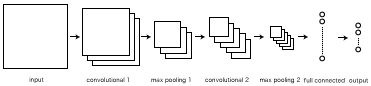
\includegraphics[width=120mm]{img/c3/convnet}
 \caption{最大値蓄積レイヤーを取り入れた畳み込みネットワーク}
 \label{c3_convnet}
\end{figure}

\subsection{DropoutとDropConnect}
\label{c3_dropout}
Dropoutとは、2012年にHinton氏らによって提案された、過学習を防ぐための技術である\cite{hinton2012improving}。過学習とは、機械学習全般において使われる用語で、学習モデルが訓練中に見たデータへの適応を重視し過ぎたために、未知のデータをうまく識別できなくなる現象のことを指す。Dropoutでは、過学習を防ぐため、各レイヤーからの出力をランダムに消去してしまう。これによって各ユニットには、他のユニットに頼らず自力で学習をする必要が生じ、より様々な入力に対応しやすい堅固(頑堅)なモデルが獲得される、と考えられている。図\ref{c3_dropout_timit}は、\cite{hinton2012improving}より引用した図で、音声認識のTIMITデータベース\cite{fisher1986darpa}\footnote{\url{http://catalog.ldc.upenn.edu/LDC93S1}}に対する識別精度である。Dropoutを使うことで、使わなかった場合に比べ、特にEpoch数(学習の繰り返し回数)が大きい場合に、分類誤差を減少出来ていることがわかる。
\begin{figure}[tbp]
 \centering
  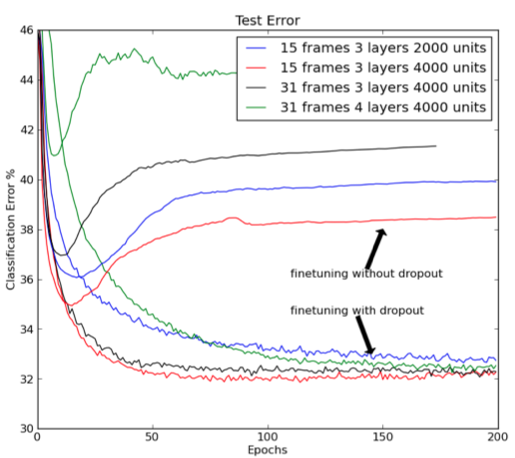
\includegraphics[width=100mm]{img/c3/dropout_timit}
 \caption{DropoutによるTIMITデータベースの識別結果}
 \label{c3_dropout_timit}
\end{figure}
\par
DropConnectは、Dropoutをさらに一般化した手法である。DropConnectでは、各ユニットからの出力ではなく、ユニット同士のつながりをランダムにカットしている。図\ref{c3_dropconnect}は、DropConnectの著者による紹介ウェブページ\footnote{\url{http://cs.nyu.edu/~wanli/dropc/}}に掲載されている画像の引用である。ニューラルネットワークにおけるニューロン同士の接続が、ランダムに切断されている様子を表している。
\begin{figure}[tbp]
 \begin{center}
  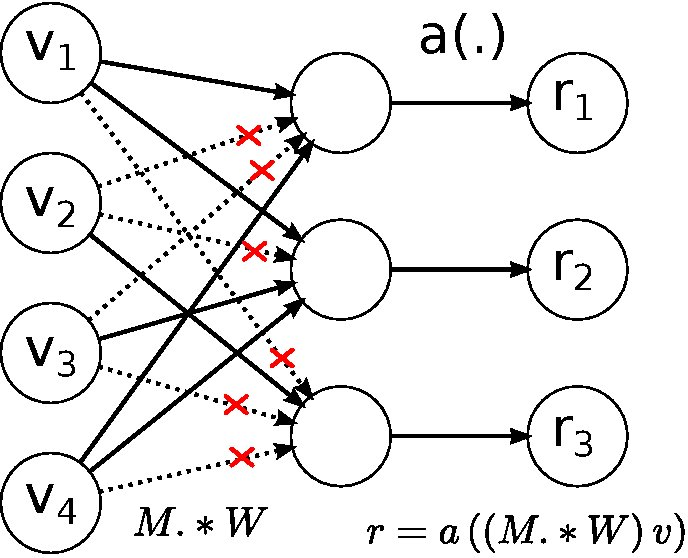
\includegraphics[width=50mm]{img/c3/nn_dc}
 \end{center}
 \caption{DropConnectの模式図}
 \label{c3_dropconnect}
\end{figure}

\subsection{活性化関数}
各ユニットに入力された値は、ある一定の関数によって増幅・変換される。これは人間の神経細胞を真似た仕組みで、神経細胞の化学物質による活性化にちなんで、活性化関数(activation function)と呼ばれる。この項では、ニューラルネットにおける様々な活性化関数を紹介する。
\subsubsection{heaviside関数}
始めにニューラルネットワークの活性化関数として用いられたがヘビサイドの階段関数である。この関数は負値に0、正値に1を返す。数式では、
\begin{equation}
H(x)= \left\{\begin{array}{cc} 0\quad (x < 0)\\ 1 \quad (x > 0)\end{array}\right.
\end{equation}
となる。ただし、これだけでは$x=0$の点で不連続になるので、$H(x)=0$や$H(x)=0.5$などの定義が用いられる。ヘビサイド関数のグラフを\ref{c3_heaviside}に示す。\par
heaviside関数は、ニューロンが受けた刺激の総和を測り、閾値を超えていれば次のニューロンにも情報を伝達し、超えていなければ何もしないという性質を、そのまま表現している。しかし、この関数は微分不可能なため、バックプロパゲーションを行う上では不都合であり、特に深層学習のネットワークモデルにおいて使われることは少ない。
\begin{figure}[tbp]
 \centering
  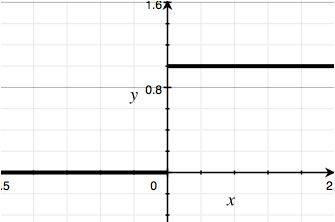
\includegraphics[width=80mm]{img/c3/heaviside}
 \caption{ヘビサイドの階段関数}
 \label{c3_heaviside}
\end{figure}

\subsubsection{シグモイド関数と双曲線正接}
シグモイド関数は、ヘビサイド関数に似ているが、全域にて非線形かつ微分可能である。この2つの特性により、バックプロパゲーションに適している。以下の式で表される。
\begin{equation}
S(x) = \frac{1}{1+e^{-x}}
\end{equation}
また、微分した形が同じシグモイド関数で表されるという特徴があり、実装が容易である。
\begin{eqnarray}
\frac{d}{dx}S(x) &=& \left( \frac{1}{1+e^{-x}} \right) \left( \frac{-e^{-x}}{1+e^{-x}} \right)\\
&=& S(x)(1-S(x))
\end{eqnarray}
シグモイド関数のグラフが図\ref{c3_sigmoid}である。ヘビサイド関数を$x=0$の付近のみ滑らかにしたような形をしている。この関数は、xの絶対値が大きくなるにつれ、yの変化が非常にに小さくなっている。そのため、ユニット間伝達において、入力と重みの積が大きくなってしまうと、その部分は誤差のバックプロパゲーションに対する反応が小さくなってしまい、学習が進みにくくなってしまうという弱点がある。
\begin{figure}[tbp]
 \centering
  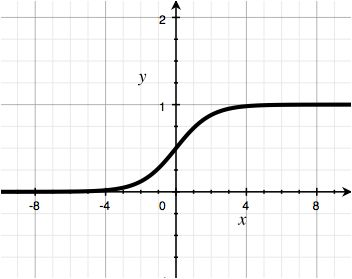
\includegraphics[width=80mm]{img/c3/sigmoid}
 \caption{シグモイド関数}
 \label{c3_sigmoid}
\end{figure}
なお、双曲線正接関数、通称tanh関数を用いることもある。シグモイド関数とtanh関数は線形の差しかないため、ニューラルネットワークの性能という面では、どちらを使用しても等価である。
\begin{equation}
tanh(x) = \frac{e^x-e^{-x}}{e^x+e^{-x}} \\\\
\end{equation}
\begin{equation}
S(x) = \frac{tanh(x/2)+1}{2}
\end{equation}

\subsubsection{整流 ユニット}
整流関数は、最近のニューラルネットワークにおいてよく用いられている活性化関数である。
\begin{equation}
f(x) = max(0, x) = \left\{\begin{array}{cc} 0\quad (x < 0)\\ x \quad (x > 0)\end{array}\right.
\end{equation}
整流関数が性能向上に役立つ理由は、まだ解明されていない。

\begin{figure}[tbp]
 \centering
  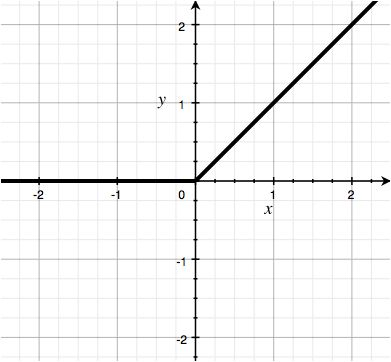
\includegraphics[width=80mm]{img/c3/rectifier}
 \caption{整流関数}
 \label{c3_整流}
\end{figure}

\subsubsection{Maxout ユニット}
Maxout Networkとは、バックプロパゲーションを伴う単純な多層MLP構造に、\ref{c3_dropout}で述べたDropout法を組み合わせ、さらにMaxout ユニットという特殊な活性化関数を併用したニューラルネットワークである\cite{goodfellow2013maxout}。Maxout Networkの1レイヤー分の構造を、図\ref{c3_maxout_arch}に示す。\par
Maxout ユニットでは、複数の線形ユニットの出力について、maxを取っている。これにより、任意の凸関数を近似することが出来る。図\ref{c3_maxout_app}は、Maxout ユニットが凸関数を近似する様子を、1次元の入力について示している。そして、複数のmaxout unitの線形和を取ることは、複数の近似された凸関数の線形和を取ることである。これによって、最終的に任意の連続関数を近似できることが証明されている。
\begin{figure}[tbp]
 \begin{center}
  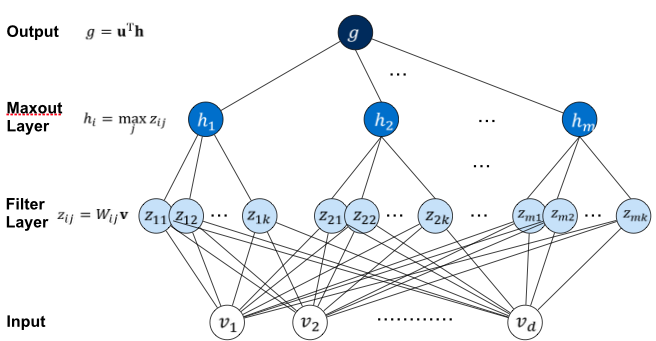
\includegraphics[width=100mm]{img/c3/maxout_arch}
 \end{center}
 \caption{Maxout Networkの構造図}
 \label{c3_maxout_arch}
\end{figure}
\begin{figure}[tbp]
 \begin{center}
  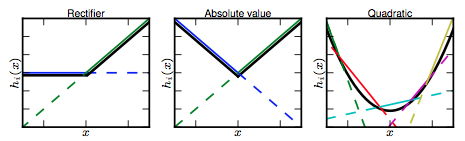
\includegraphics[width=100mm]{img/c3/maxout_app}
 \end{center}
 \caption{Maxout ユニットが凸関数を近似する様子(1次元の場合)}
 \label{c3_maxout_app}
\end{figure}

% !TEX root = thesis.tex
\chapter{深層学習の実装における課題とその対策の提案}
この章では、まず深層学習のアルゴリズムを実装する際に起こり得る、様々な問題点について整理する。次に、様々な問題点を解決するため、開発者が採ることの出来る対策について詳しく考察する。考察の一部では、実際のソースコードによる実証実験が必要となる。この実験については、5章にて詳しく述べる。

\section{深層学習の実装における問題点}
深層学習のアルゴリズムを、ウェブ工学などに応用するための具体的な実装を行う際の問題点として、次の3つの問題が考えられる。
\begin{itemize}
\item \textbf{分類精度の再現の問題}。 深層学習が注目された大きな理由である、高い識別精度を実現できるアルゴリズムかどうか。また、論文において掲げられている精度を再現できる実装を手元に用意したり、あるいは制作できるかどうか。
\item \textbf{実装難易度の問題}。実際の問題に応用するにあたって、必要なプログラミング技術や数学的知識は、出来るだけ低くて済む方が望ましい。
\item \textbf{学習時間の問題}。深層学習では、 学習にかかる時間が非常に長くなることがある。グラフィックスプロセッシングユニット(Graphics Processing Unit、以下GPU)を用いることで実行速度を上げることが出来るが、GPUを利用するための実装自体も難しい。これは、実装難易度の問題とも関連する。
\end{itemize}
以下、これら3つの問題について、詳しく述べる。

\subsection{分類精度の再現の問題}
今回深層学習を選択した理由は、ウェブ工学のタスクにおいて、高い分類精度を実現するための最も有力な方法だと思われるからである。逆に、深層学習の分類精度が従来の分類器より劣っているならば、従来の分類器を使った方が望ましいと言える。\par
アルゴリズムを紹介する論文では、対応する実装が公開されていなかったり、例えメインのアルゴリズムについては書いてあっても、実験の際に設定したハイパーパラメータの詳細について記していない場合がある。ハイパーパラメータの値や決め方が公開されていない場合、自ら全てのコードを実装したり、問題に応じてアルゴリズムの細部やハイパーパラメータを柔軟に調整しなければならない場合もある。利用者が実装したり手を加えたソースコードでは、論文の著者と正確に同じモデルやアルゴリズムを使用できているのかどうかが不明である。よって、本当に論文に記述してある性能が発揮できるのかどうか、実際に利用してみないとわからない。この問題は、論文で扱っていない新しい入力データを扱う場合により顕著になると考えられる。なぜなら、初めてのデータにおいては、仮に論文のものと細部まで等しいアルゴリズムを実装できたとき、どの位の分類精度が実現できるのかわかっていないため、アルゴリズムの精度面での正しさを検証することが出来ないからである。\par

\subsection{実装難易度の問題}
この問題は、主に標準といえる公開ライブラリが確立していないことが原因である。深層学習は歴史の浅い発展途上の技術であり、どのアルゴリズムを定番とすれば良いのか、試行錯誤の段階にある。各アルゴリズムの改良点が次々と見つかっていることに加え、学習性能が高くなる原理や、学習対象に対する各アルゴリズムの得手不得手など、解明中の部分も多い。アルゴリズムが開発途上で確定できていないため、公開されているライブラリも、現状では、開発用途や実験的なものが多くなってしまっている。実験的なライブラリでは、一部の種類のデータに対する学習のみを想定している場合があり、この場合他の種類のデータを扱うためには、データ変換用のソースコードを記述しなければならない。\par%標準ライブラリがある分野、例えばLIBSVMやmatlabの制御系、excelの統計は利用が簡単なことに言及
手元のパソコンにて実行可能な深層学習のソースを探し当てたとしても、このソースが実際に、論文にて示されているような高い精度を実現できるかどうかは、実際のデータを当てはめてみるまで定かではない。これは先ほど述べてように、まだアルゴリズムの細部が固まっておらず、実装ごとにバリエーションが大きいためである。また、ソースコードが言わばお試し用の状態になっていて、単にアルゴリズムの要点を示すためのものだったり、実行時間の短縮を重視したハイパーパラメータの調整が為されていて、論文に記述してある精度を実現できないこともある。\par
このようにライブラリが確立していない状況では、プログラマが自ら深層学習のコードを記述する必要がある。しかし、深層学習の原理は多くの数学的背景の下成り立っており、理解には多くの時間がかかる。結果としては、プログラム開発に長い時間がかかってしまい、ビジネスシーンにおいて不利であると考えられる。なおライブラリの未成熟さや、実装・改造の難しさは、自力実装における「分類精度の再現の問題」にも影響している。\par

\subsection{学習時間の問題}
深層学習のモデルを訓練するには、無視できない長さの時間が必要となる。例えば、先述したGoogleによるSupervisionの学習では、1000台のマシンによるクラスタを用いても、訓練に3日間かかっており、個人レベルでは実験自体がほぼ不可能である\cite{le2012building}。一回の学習の時間が長くなれば、それだけ技術開発にかかる時間も長くなり、刻一刻と変化するウェブサービスに対して応用するのは難しくなる。特に、スタートアップ企業が深層学習の技術を用いて市場での優位を得ようとする場合を考えると、開発期間の短縮は大きなポイントである\cite{ries2011the-lean}。\par
必要実行時間の長さをカバーするため、GPUを用いて演算をスピードアップさせる手法が確立されつつあるが、GPUは比較的高価なパーツである上、GPUの利用には特殊なプログラミングが要求され、開発における障壁の1つとなっている(つまりこれは「実装難易度の問題」でもある)。また、大部分のノートパソコンや一部のサーバなど、並列演算に利用可能なGPUの搭載自体が出来ないパソコンを使っている場合ではGPUを利用しているソースコードの実行が全く出来ないこともある(後述)。\par

この章の残りでは、今挙げた「分類精度の再現の問題」「実装難易度の問題」「学習時間の問題」を解決するための方策について述べる。ただし、「分類精度の再現の問題」については、最終的にソースコードを実行してみないと、再現性が確保されていることを確かめられない。そこで、「分類精度の再現の問題」については、5章にていくつかのアルゴリズムや実装による実験を行うことで、更なる検証を行う。

\section{実装上の問題への対策}
ここでは、前節で述べた3つの実装における問題点のそれぞれに対して、開発者がどのような対策を採れるのか、考察する。また、これらの3つの問題点の全てに共通して、「適切なライブラリの組み合わせを選択する」という対策が有効である。これについては、最後にまとめて言及する。
\subsection{分類精度の再現の問題への対策}
「分類精度の再現の問題」は、論文だけでは実装に必要な全ての情報が得られないことが原因である。これを解決する最も簡単な手段は、論文やアルゴリズムの中で、実際に分類実験に用いたソースコードをそのまま提供しているものを選び、そのソースコードを出来るだけ変更せずに使うことである。
\begin{figure}[tbp]
 \begin{center}
  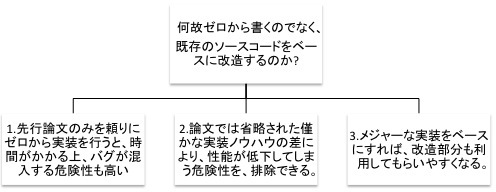
\includegraphics[width=120mm]{img/c4/library_merit}
 \end{center}
 \caption{既存コードの利用における、完全オリジナルコードの作成に対する利点}
 \label{c4_library_merit}
\end{figure}
深層学習のプログラムを実装するために、まず大きく分けて、「自分でソースコードを全て書く」方法と、「主に既存のソースコードを利用する」方法の2つが考えられる。「既存のソースコードを利用する」場合のメリットとして、「開発期間は基本的にゼロで済む」「新たにバグが混入する危険性が無い」「自分の改造コードが、他のライブラリ利用者によって使ってもらえるチャンスが大きい」という点が挙げられる(図\ref{c4_library_merit}参考)。デメリットとして、「ソースコード中にブラックボックスが増え、改造にかかる時間が短くなる」「全く新しいアルゴリズムを実装する場合、ゼロからスタートした方が早く書けるケースもある」などが想定される。しかし、分類精度を再現できる可能性を高くするため、今回は既存のソースコードを探して利用していくことにした。既存ソースコードを利用する際に生じるリスクについては、図\ref{c4_library_hedge}のように対処できる。\par
\begin{figure}[tbp]
 \begin{center}
  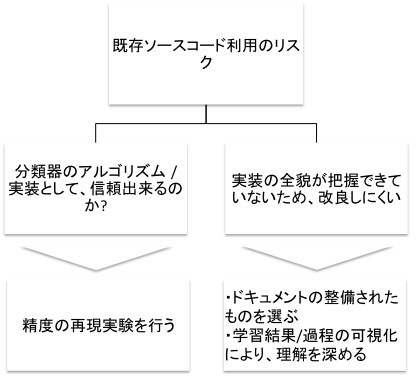
\includegraphics[width=90mm]{img/c4/library_hedge}
 \end{center}
 \caption{既存ソースコード利用のリスクと、対処方法}
 \label{c4_library_hedge}
\end{figure}
なお、「自分でソースコードを全て書く」場合のメリットとデメリットは、上記「既存のソースコード」の場合の逆となる。自分で新たなコードを書くので時間がかかり、バグの混入リスクも大きい。また、ソースコードを公開した場合の、ライブラリとしての信頼度も、ゼロから築かなければならない。ただし、コードの詳細部分を改造して、深層学習の新たなアルゴリズムを開発する段階に至った研究者にとっては、自分の手で書いたコードを使う方が、より深い理解を得やすく、確実で素早い実装ができる可能性もある。

\subsection{実装難易度の問題への対策}
「分類精度の再現の問題」でも挙げた、既存のソースコードを利用することが、「実装難易度の問題」に対する直接的な解決方法の1つにもなる。深層学習のアルゴリズム自体が改良の過程で単純な数学的モデルへと帰着し、実装が容易になる可能性も否定できないが、ここでは現段階で採れる方策のみを考えるということで、除外する。\par
ただし、実装難易度を下げるという観点からは、「分類精度の再現の問題」を解決できるだけでなく、さらにソースコードの利用や解読・改造が容易であることが重要である。ソースコードの改造については、もちろん全くしないで済むのが理想ではある。しかし実際には、現在の深層学習のアルゴリズムで、細部の調整なしに良い結果を出すことは難しい。よって応用開発ではいくらかのプログラミングが必要となることが予想される。このときソースコードの読みやすさや改造のしやすさは重要な長所となる。また、ソースコード開発コミュニティが活発であれば、自分以外の開発者がソースコードの問題点やバグを修正してくれる可能性が出てくる。開発上で生まれた疑問が、コミュニティの構成員によって解決してもらえることもあるため、実装の助けとなる。\par%オープンソース
深層学習に利用できるライブラリは、まだ標準が固まっていないものの、論文と共にソースコードを公開するパターンが多く、いくつか出回っている。どのようなライブラリが存在するかについて、次の節にて詳しく述べる。


\subsection{学習時間の問題への対策}
学習時間を短縮するためには、アルゴリズム自体の改良が最も重要であるが、もちろんその難易度は高い。ここでは、アルゴリズムを実行するハードウェアに着目し、特に近年盛んになっているGPUの利用による高速演算、GPUコンピューティングに焦点を当てる。
\subsubsection{GPUの利用による高速化}
GPUとは、CPUと併用できるプロセッサの一種で、主に画像処理演算を担当している。GPUは元々、画像処理に必要な行列演算などを、CPUよりも効率良く扱えるように開発された。現代のGPUは、単にグラフィック処理に特化したプロセッサというだけでなく、その並列演算能力を活かして、大量の演算を行う科学計算用途にも使われている。GPU設計・製作メーカーのNVIDIAからは、グラフィック出力機能を敢えて外し、科学計算用途に特化した、TeslaというハイエンドGPUシリーズも発売されている\footnote{\url{http://www.nvidia.co.jp/object/tesla-supercomputing-solutions-jp.html}}。\par 
深層学習の研究においても、GPUによる並列計算が有効とされている。これは、入力ベクトルと重み行列の積など、ニューラルネットワークの計算にて中心を占める行列演算が、並列計算の恩恵を受けやすいからである\cite{bengio2012practical}。例えば、前述したDropConnectの研究\cite{wan2013regularization}に拠れば、GPUで演算した場合、テクスチャメモリを利用しなくてもCPUより97.2倍高速化でき、テクスチャメモリを利用すれば414.8倍の速度を出すことも可能である。\par
また、深層学習の実装によっては、はじめからGPUで高速化することを前提に、GPU専用のコードを書いている場合がある。例えば、後述するcuda-convnet\footnote{\url{https://code.google.com/p/cuda-convnet/}}や、Maxout Network\cite{goodfellow2013maxout}のコードの一部、DropConnect\cite{wan2013regularization}\footnote{\url{http://cs.nyu.edu/~wanli/dropc/}}が該当する。この場合、そもそもGPUを搭載したマシンを使わないと、コンパイルや実行が全く出来なくなってしまう。\par
%CPUの計算能力は頭打ちになっている。
GPUが高速に演算を実行できる理由は、その構造にある。1〜数個のプロセッサで様々な命令をこなすCPUに対し、GPUは数百〜数千個のcoreを持っており、同一の命令を高速に並列演算する用途に向いている。これは、大量の点の変換処理が必要となるグラフィック処理環境から生まれたGPUの強みである。かつてGPUを科学演算に用いるには、OpenGL\footnote{\url{http://www.opengl.org/}}やCg\footnote{\url{http://www.nvidia.co.jp/object/cg_jp.html}}のようなグラフィック処理用ライブラリを使ってアルゴリズムを記述しなくてはならず、非常に難易度が高かった\footnote{\url{http://www.nvidia.co.jp/object/what-is-gpu-computing-jp.html}}。そこで、NVIDIAはCUDAというGPUによる演算の開発環境を開発した\cite{garland2008parallel}。CUDAはC/C++言語を拡張した作りになっており、グラフィックライブラリに比べて記述は非常に容易である。また、PythonにてCUDAコードを生成するライブラリも存在している\cite{kloeckner2009pycuda:}\cite{klockner2012pycuda}。\par
GPUによる並列演算は高速だが、GPUのメモリとCPUのメモリとの間で起こる通信は、比較して低速であり、ボトルネックになることが多い。通信の回数を減らし、GPU上のみで完結する演算を増やすことが重要である\cite{bengio2012practical}。

\subsubsection{GPUの選定}
前項で述べた通り、深層学習を高速に行うためには、GPUの応用が重要である。ここでは、機械学習を行うマシンに搭載するGPUを、選ぶときのポイントについて記す。\par
まず、GPUは、NVIDIA製で、CUDAに対応していなければならない。ただし、グラフィック出力の機能はなくても構わない。\par2013年1月現在、NVIDIAのウェブページに掲載されているGPUに関しては、全てCUDAに対応しているため、店舗で新品のGPUを購入する場合は基本的に問題は生じないと思われる。\par
なお、NVIDIAと並ぶGPUの開発メーカーであるAMD社も、CUDAと同様のGPUコンピューティング支援システムであるATI Streamという技術を開発している\footnote{\url{http://www.amd.com/jp/products/technologies/stream-technology/Pages/stream-technology.aspx}}。しかし、現在深層学習にて使われているライブラリは、後述するようにCUDAをベースとしているものが多いため、ここではCUDAの利用のみを前提として考える。\par
NVIDIAのGPUの中で、どれを選ぶかも問題になる。NVIDIAのウェブページでは、GPUのうちTeslaというシリーズがGPUによる科学演算や高品質な画像生成に特化しており、非常に高精度/高速な演算を行うことができる、と述べられている。しかし、非常に高価な上、Teslaシリーズは一般的なタワー型PC向けのグラフィックカードではなく、大型サーバやワークステーションでの利用を基本としている\footnote{\url{http://www.nvidia.co.jp/object/tesla-servers-jp.html}}\footnote{\url{http://www.nvidia.co.jp/object/where-to-buy-tesla-jp.html}}。専門家の方によれば、Teslaは主に商用の大規模データや、ミスの許されない長時間科学計算などに用いることを想定して作られている。今回の目的は、ウェブ工学の一般的タスクにおける深層学習技術を確立するという、いわば実験的な用途であり、Teslaの利用はオーバースペックだと思われる。\par
NVIDIAのGPUは、Teslaを除くと、QuadroとGeForceという2つのシリーズに分かれている。専門家の方に詳しい話を伺ったところ、Quadroはコンピュータグラフィックの出力機能に注力したシリーズであり、GeForceはより計算性能重視という傾向をもっている。つまり、深層学習の計算などGPGPUに用いる場合、同じ価格帯ならば、GeForceシリーズのGPUを用いた方が、費用対効果が大きくなると考えられる。\par
また、専門家の方によれば、GeForceシリーズの中でもTitanという機種は、Tesla用の部品の中で品質チェックに漏れてしまったものを流用しており、Teslaとほぼ同様の、非常に高い性能を発揮することが出来る、とのことだった。しかし、今回利用する中で最も計算量が大きいMaxout Networkについて、元の発表論文によれば、GeForceシリーズのGTX 580という、少し世代が前のGPUが用いられている。深層学習を実行させる上で、GPUが存在すること自体は非常に重要だが、必ずしも最新スペックのGPUが必要というわけではないことがわかる。


\subsection{深層学習に応用できるライブラリ}
「分類精度の再現の問題」「実装難易度の問題」で述べたように、深層学習の実装においては、分類性能が高く、かつ利用が容易な公開ライブラリを選ぶことが重要となる。また、「学習時間の問題」で述べたように、現段階で学習時間の短縮に最も有効な手段の1つが、GPUの利用であり、GPU用のコードを記述するためにもライブラリが重要である。つまり、深層学習の実装では、適切なライブラリを選択することが重要となる。そこで、この節では現在深層学習を実装する際に利用できるライブラリやソースコードを紹介する。

\subsubsection{cuda-convnet}
CUDAとC++による畳み込みネットワークの実装が、CIFARデータセットの制作者であるKrizhevsky氏によって公開されている\footnote{\url{https://code.google.com/p/cuda-convnet/}}。最大値蓄積レイヤーや最終レイヤー用のソフトマックスレイヤーなど、畳み込みネットワークの実装に必要なパーツが一通り用意されている。なお、後述するPylearn2にも、このcuda-convnetのPythonラッパクラスが実装されている。

\subsubsection{word2vec}
1章で紹介した、単語をベクトル化するword2vecのコードも全て公開されている。また、ウェブアプリにもなっており、誰でもブラウザ上でテキストデータを入れるだけで、意味ベクトルを生成できるようになっている\footnote{\url{https://code.google.com/p/word2vec/}}。word2vecは、入力されたテキストデータから、まず単語の辞書を作り、次にそれぞれの単語の意味をベクトル化していく。ベクトル化が済めば、単語同士の類似度を計測したり、クラスタリングに用いることができる。

%\subsection{DropConnect}
%DropConnectのソースコードも、ウェブページにて公開されている。CUDAとC++を用いた独自のコード
%sentiment analysis
%torch7
%sugomori
%nolearn
%deepnet
%scikit
%pycuda
%hinton(matlab)

\subsubsection{数値計算ライブラリTheano}
Theanoは、python上で記述される数式処理/数値計算ライブラリである。Theanoは、数式のコンパイルと実際のデータによる数値計算の2段階で動作する\cite{bergstra2010theano:}。図\ref{c4_Theano_compile}に、Theanoが動作する仕組みを示した。
\begin{figure}[tbp]
 \centering
  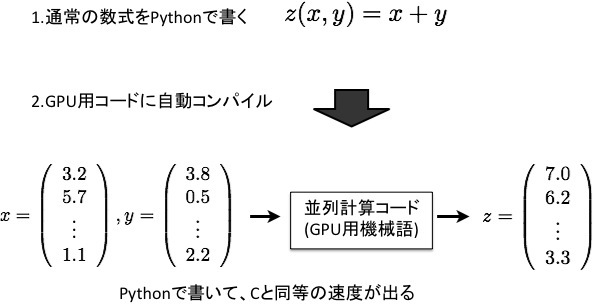
\includegraphics[width=120mm]{img/c4/theano_compile}
 \caption{Theanoの動作過程}
 \label{c4_Theano_compile}
\end{figure}
Theanoでは、数式は文字シンボルを用いた文字式で記述できる。記述された文字式は、内部的には計算木(グラフ)として蓄積されている。Theanoは、実際の計算を行う前に、このグラフをコンパイルして、CによるCUDAのコードに変換している。このときデバッグの難しい数値計算の誤差絡みの部分、0による除算など危険な処理を、自動的に解析してくれる。ニューラルネットワークの演算過程では、非常に小さい数値が出現することがあり、また、文字式を分析することで、計算グラフも最適化してくれる。プログラマは、プログラム上の些末な計算テクニックに囚われることなく、数式の本質的な部分の記述に集中することができる。また、記号ベースの解析的な微分を自動で行ってくれる機能がついている。この記号微分機能は、ニューラルネットワークの実装において大いに助けとなる。ニューラルネットワークでは、バックプロパゲーションを実装するため、モデルを構成する大量のパラメータにて、損失関数を微分する必要がある。ネットワークが多層になるとパラメータ数も増加し、微分の計算式はさらに複雑になる。微分計算を最適化するため、手計算による文字式の微分をしてから実装を行うと、層を増やす度に非常に煩雑な手計算が必要であり、開発効率の低下は避けられない。Theanoの自動微分と自動最適化は、深層学習のアルゴリズムを簡略に記述するための、大いなる助けとなる。

\subsubsection{Deep Learning Tutorial}
Deep Learning Tutorialは、Theanoを用いて記述されたソースコードで、Theanoと同じくLISA.研究室のメンバーによって書かれている。内容的には、単純なロジスティック回帰から始まり、最終的に畳み込みネットワーク, 積層雑音除去自己符号器, 深層信念ネットワークの3つの原理が理解できるよう構成されている。ソースコードのほぽ全ての部分に、詳細なコメントが書いてあり、深層学習のアルゴリズムと同時にTheanoを用いた実装上の注意点なども理解できるような作りになっている。\par
一方で、提供されているコードは簡単のため、アルゴリズムの基本的な部分に絞られており、最新の研究成果が反映されているわけではないため、注意が必要である。例えば、畳み込みネットワークのソースコードには、1998年のLeCunらによる研究\cite{lecun1998gradient-based}をベースにしていると書いてある。しかし、元の論文の段階で既に、2012年に発表された最も優れている畳み込みニューラルネットワーク\cite{ciresan2012multi-column}に比べて、3倍以上誤差が大きくなってしまっている。またあくまでTutorialという位置づけのため、繰り返し回数などのハイパーパラメータが最も誤差が低くなるようには設定されていない。\par
なお、深い構造の形にはなっていないが、雑音除去自己符号器の代わりとして、契約自己符号器\cite{rifai2011contractive}\cite{rifai2011learning}の実装も提供されている。これは、雑音除去自己符号器の亜種だが、誤差測定時に適切なベナルティ項を与えることで、学習される表現の頑健性がさらに向上するというものである。

\subsubsection{機械学習ライブラリPylearn2}
Pylearn2は、pythonで記述された、深層学習など機械学習アルゴリズムを使うためのライブラリである\cite{goodfellow2013Pylearn2:}。やはりモントリオール大学のLISA.研究室の方がメインとなっており、github上でソースコードの更新がほぼ毎日行われている。以下、Pylearn2の特徴を記す。
\begin{itemize}
\item \textbf{高精度アルゴリズムMaxout Networkの実装}
Pylearn2には、3章にて述べた、Maxout Networkという深層学習のアルゴリズムの一種が実装されている。このアルゴリズムは、画像認識タスクにおいて非常に高い精度を実現しており、高い分類精度を満たせる可能性が高い。
\item \textbf{Theanoの利用}
Pylearn2のプログラムは、前述したTheanoを全面的に利用して記述されている。Theanoを用いたことで、可読性が大きく上昇している。
\item \textbf{高度な拡張性と可読性}
Pylearn2のソースコードは、拡張性や可読性を非常に強く意識して書かれている。基本的な使い方を記したチュートリアルのウェブページが存在し、主なソースファイルには、詳細なドキュメントも記述されている。また、モジュール化が丁寧なので、自分で書く部分が少なくて済む。例えば、データセットを変更する場合は、Datasetクラスのみを書き下せばよく、他の部分に対してコードを書く必要がほとんどない。図\ref{c4_Pylearn2_yaml}に、Pylearn2において機械学習のアルゴリズムがどのようにモジュール化されているかを示す。\par
また、プログラムを改造する場合でも、数値パラメータを変更するだけであれば、設定ファイルのみの変更で完結させることができる。この設定ファイルは、YAML(YAML Ain't a Markup Language)形式に少し独自拡張を加えた形式になっている。\par
プログラム本体と、数値の設定ファイルが分離されていることで、プログラミングが不得手な人でも、比較的簡単に設定を変更することができる。\par
\begin{figure}[tbp]
 \begin{center}
  \includegraphics[width=120mm]{img/c4/Pylearn2_yaml}
 \end{center}
 \caption{Pylearn2の実験計画例}
 \label{c4_Pylearn2_yaml}
\end{figure}
\end{itemize}
\begin{comment}
\subsubsection{Pylearn2の主なパッケージ}
現在のPylearn2のソースコードは、使われているものと非推奨のものが混在している。これは、Pylearn2に定められたAPI変更のルールのためである。Pylearn2では、「変数やクラスを消去する半年前に、ライブラリ上で告知しなければならない」という管理方針を定めている。これは、Pylearn2の安定性に寄与しているが、一方で、ソースコードリーディングの際には使われていないパッケージがノイズになることも少なくない。ここでは、Pylearn2で現在使われている主なパッケージについて紹介する。
\begin{itemize}
\item \textbf{costs} 最終レイヤーで誤差を計算するときに使われる、損失関数(loss function)を集めたパッケージである。主にSGDによって利用される。Dropout、Lpペナルティ、クロスエントロピー関数、負の対数尤度関数などがここに含まれている。また、DBNや自己符号器のように、独自の損失関数が必要な場合も、ここで定義されている。
\item \textbf{datasets} MNISTやCIFAR10, SVHNなどのデータセットがクラス化されている。新しいデータセットに対して深層学習を使いたい場合は、ここに定義されているDatasetクラスやDenseDesignMatrixクラスのサブクラスを作成することになる。
\item \textbf{distributions} ガウス分布などの分布関数が集められている。
\item \textbf{gui} 主に重みフィルタを可視化するためのクラスが用意されている。
\item \textbf{linear} Theanoの線形変換クラスを作り直したもので、畳み込みレイヤーもここに含まれる。
\item \textbf{models} 自己符号器、RBMなどの学習モデルが定義されている。
\item \textbf{sandbox} cuda-convnetのラッパクラスが定義されている。
\item \textbf{scripts} 実際に学習を行わせたり、学習結果を集計するときに便利なスクリプトが集められている。
\item \textbf{train\_extensions}学習がスタートする時や、1回の処理が終了したときに動かす処理を定義するためのクラスである。デザインパターン\cite{gamma1995design}でいうObserverパターンが用いられている。
\item \textbf{training\_algorithms} SGDとバッチ勾配降下法を始めとする、学習アルゴリズムが定義されている。SGDと併用するための、学習率変化アルゴリズム(線形減少、指数関数的減少、焼き鈍し)、慣性率の利用、Polyak平均化\cite{polyak1992acceleration}なども、ここで一緒に定義されている。


\end{itemize}
\end{comment}
% !TEX root = thesis.tex
\chapter{ウェブ工学への深層学習技術の応用}
この章では、第4章で得られた深層学習用の構成を用いて、実際に機械学習のタスクを実行する。分類精度、実行時間、消費メモリ量を調べることにより、深層学習をウェブ工学の問題に適用する際の参考とする。
\section{利用したデータセット}
実験の前提知識として、この節では、実験に使用したデータセットについて記す。機械学習の分野では、分類精度のベンチマークを取るために、様々なデータセットが提供/提案されてきている。同じデータセットに対して、様々な分類モデルやアルゴリズムを用いて分類実験を行うことにより、どの手法が優れているのか比較することが出来る。\par
ここでは、画像認識のデータセットを用いて、深層学習プログラムのベンチマークを行う。画像データを用いる理由は、1つには、画像認識が深層学習が最も高い分類性能を実現している分野だからである。加えて、画像データや画像から抽出された素性は、可視化が比較的容易なことが多い。可視化することで、学習過程を目で見て確かめることが出来るため、アルゴリズムの分析を行いやすい、という利点がある。
\subsection{MNIST}
MNIST database\footnote{http://yann.lecun.com/exdb/mnist/}とは、手書き数字を画像分析によって認識するベンチマークタスクである。このデータセットは、National Institute of Standards and Technology(NIST)が提供する手書き数字のデータにサイズの規格化処理を加え、数字の書き手毎に整理したものである。データはサイズ28x28ピクセルの白黒画像70000件より構成される\cite{lecun1998gradient-based}。それぞれの画像は、0〜9のいずれかの数字1文字に該当している。画像データを認識プログラムに入力して、どの数字に該当するか判別させることで、画像識別の精度を競うことになる。図\ref{c5_mnist_ex}に、MNISTの画像データの一部を示す(\cite{lecun1998gradient-based}より引用した)。\par
MNISTの70000件のデータは、60000件のモデル訓練用データと、10000件の精度測定用データに分かれている。まず60000件のデータを使って識別モデルに学習を行わせた後、未知の10000件のテストデータを実際に識別してみることで、精度を測定する。テストデータを識別している最中に、更なる学習を行うことは許されない。分類器は、過去に学習に使ったデータだけ良く識別できても意味がなく、むしろ未知のデータこそ精度良く分類出来なければならない。モデルが過去のデータに特化してしまうと、かえって未知のデータに対する識別精度が低下することもある。この低下現象は過学習(over fitting)と呼ばれ、機械学習における落とし穴の一つとなっている。MNISTに限らず、機械学習用のデータセットにて、訓練データとテストデータをあらかじめ分けておくことは一般的であり、学習アルゴリズムが過学習を防げているかどうか、判定するために有効な方法の1つとして知られている。\par
\begin{figure}[tbp]
 \begin{center}
  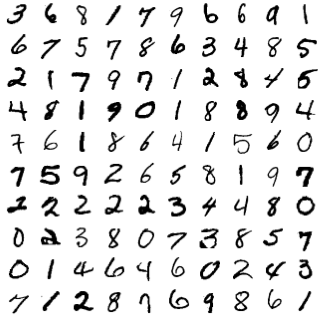
\includegraphics[width=50mm]{img/c5/mnist_ex}
 \end{center}
 \caption{MNISTデータの例}
 \label{c5_mnist_ex}
\end{figure}
MNISTは、様々な画像認識アルゴリズムの作者によって使用されている。MNISTの配布ウェブサイトには、MNISTを利用した論文のリストが、分類誤差によるランキング形式で掲載されている。表\ref{c5_mnist_rank}に、MNISTデータセットにおける各アルゴリズムの分類誤差を、ランキング形式のウェブサイト\footnote{\label{c5_rank}\url{http://rodrigob.github.io/are_we_there_yet/build/classification_datasets_results.html}}より再構成して示す。

% Table generated by Excel2LaTeX from sheet 'c5mnist'
\begin{table}[htbp]
\begin{center}
  %\centering
  \caption{MNISTの分類誤差ランキング}
    \begin{tabular}{|l|l|r|}\hline
%    \toprule
    手法 & 発表学会/雑誌/年 & 分類誤差 \\ \hline
%    \midrule
    DropConnect \cite{wan2013regularization}& ICML 2013 & 0.21\% \\ \hline
    Multi-column 深層ニューラルネットワークs \cite{ciresan2012multi-column}& CVPR 2012 & 0.23\% \\ \hline
    Deep Big Simple Neural Nets \cite{ciresan2010deep}& Neural Computation 2010 & 0.35\% \\ \hline
    エネルギーに基づくモデル \cite{poultney2006efficient}& NIPS 2006 & 0.39\% \\ \hline
    畳み込みニューラルネットワークworks \cite{simard2003best}& Document Analysis and Recognition 2003 & 0.40\% \\ \hline
    \textbf{Maxout Networks} \cite{goodfellow2013maxout}& ICML 2013 & 0.45\% \\ \hline
    COSFIRE フィルタs \cite{azzopardi2013trainable}& PAMI 2013 & 0.52\% \\ \hline
    Multi-Stage Architecture \cite{jarrett2009what}& ICCV 2009 & 0.53\% \\ \hline
    Deformation Models \cite{keysers2007deformation}& PAMI 2007 & 0.54\% \\ \hline
    A trainable feature extractor \cite{lauer2007a-trainable}& Journal Pattern Recognition 2007   & 0.54\% \\ \hline
    Invariant サポートベクターマシンs \cite{decoste2002training}& Machine Learning 2002 & 0.56\% \\ \hline
    Sparse Coding \cite{labusch2008simple}& TNN 2008 & 0.59\% \\ \hline
    教師無し learning of invariant feature hierarchies \cite{ranzato2007教師無し}& CVPR 2007 & 0.62\% \\ \hline
    shape contexts \cite{belongie2002shape}& PAMI 2002 & 0.63\% \\ \hline
    Receptive Field Learning \cite{jia2012beyond}& CVPR 2012 & 0.64\% \\ \hline
    Sparse Activity, Sparse Connectivity \cite{thom2013sparse}& JMLR 2013 & 0.75\% \\ \hline
    Convolutional 深層信念ネットワークworks \cite{lee2009convolutional}& ICML 2009 & 0.82\% \\ \hline
    Deep Encoder Network \cite{min2009large-margin}& 2009 & 0.94\% \\ \hline
    Deep Boltzmann Machines \cite{salakhutdinov2009deep}& AISTATS 2009 & 0.95\% \\ \hline
    深層信念ネットワークworks \cite{dahl2008cs81:}& 2008 & 1.12\% \\ \hline
    畳み込みニューラルネットワークworks  \cite{simard2003best}& 2003 & 1.19\% \\ \hline
    neural networks \cite{hinton2006reducing}& 2006 & 1.20\% \\ \hline
    Deep learning via semi-教師有り embedding \cite{weston2012deep}& 2008 & 1.50\% \\ \hline
%    \bottomrule
    \end{tabular}%
  \label{c5_mnist_rank}%
  \end{center}
\end{table}%

\subsection{CIFAR10}
CIFAR10\footnote{http://www.cs.toronto.edu/~kriz/cifar.html}は、写真を画像分析によって識別するタスクである\cite{krizhevsky2009learning}。入力データは60000件のカラー画像で、どの画像も、飛行機、自動車、鳥、猫、鹿、犬、蛙、馬、船、トラックの10種類のクラスのどれかに属しており、各クラス均等に6000枚ずつの画像が割り振られている。画像データは、GoogleやFlickrなどによるウェブ検索で集められた画像を、人手でラベリングして作られている。また、サイズを32x32ピクセルに縮小されている。\par
MNISTと同じように、60000件のデータは、50000の訓練データと10000件のテストデータに分割されている。まず、分類器にこれらの訓練データを読み取らせて、学習を行わせる。その後、テストデータのうちいくつを正しいクラスに分類することができるのか、分類精度を競うことになる。\par
CIFAR10についても、データの例を\ref{c5_cifar_ex}に、分類誤差のランキングウェブサイト\footnote{\url{http://rodrigob.github.io/are_we_there_yet/build/classification_datasets_results.html}}より、再構成した表を\ref{c5_cifar_rank}に示す。
\begin{figure}[tbp]
 \begin{center}
  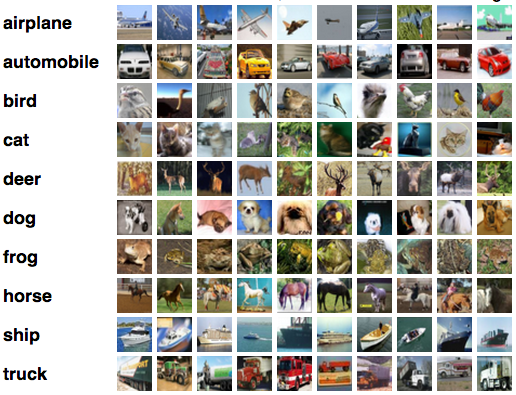
\includegraphics[width=100mm]{img/c5/cifar_ex}
 \end{center}
 \caption{CIFAR10データの例}
 \label{c5_cifar_ex}
\end{figure}
\begin{table}[tbp]
 \begin{center}
  \begin{tabular}{|l|l|r|}\hline
  手法 & 発表学会/雑誌 & 分類誤差 \\ \hline
DropConnect \cite{wan2013regularization}& ICML 2013 & 9.32 \% \\ \hline
Maxout Networks \cite{goodfellow2013maxout}& ICML 2013 & 9.35 \% \\ \hline
Bayesian Optimization \cite{snoek2012practical}& NIPS 2012 & 9.50 \% \\ \hline
Deep 畳み込みニューラルネットワークworks \cite{krizhevsky2012imagenet}& NIPS 2012 & 11.00 \% \\ \hline
Multi-Column 深層ニューラルネットワークs \cite{ciresan2012multi-column}& CVPR 2012 & 11.21 \% \\ \hline
Deep 畳み込みニューラルネットワークworks \cite{zeiler2013stochastic}& arXiv 2013 & 15.13 \% \\ \hline
Dropout \cite{hinton2012improving}& arXiv 2012 & 15.60 \% \\ \hline
Sum-Product Networks \cite{gens2012discriminative}& NIPS 2012 & 16.04 \% \\ \hline
Single-レイヤー Networks \cite{coates2011an-analysis}& AISTATS 2011 & 20.4 \% \\ \hline
  \end{tabular}
 \end{center}
 \caption{CIFAR10分類誤差のランキング}
 \label{c5_cifar_rank}
\end{table}

\section{使用したライブラリ}
この章の実験には、Pylearn2という深層学習のライブラリを用いた。
\section{使用したハードウェア}
この章の実験では、GPUを搭載したサーバマシンを用いた。表\ref{c5_hardware_spec}に、今回の実験で使用したマシンの主な使用パーツ及び性能を列挙した。また、Maxout Networkの実装ソースコードには、実験マシンのパーツ性能を書いたファイルが付属している\footnote{Pylearn2/scripts/papers/maxout/notes}。このファイルの記述内容も、比較のために列挙した。今回の実験に使ったマシンの方が、ハードウェア性能的には優れていることがわかる。
\begin{table}[tbp]
 \begin{center}
  \begin{tabular}{|c|c|c|c|c|c|}\hline
   & GPU & CUDA core & CPU & クロック数 & メモリ容量\\ \hline
今回 & GTX760 & 1152 & Intel CPU Core i7 4770S & 3.1 GHz & 32GB\\ \hline
論文 & GTX580 & 512 & Intel Xeon CPU E5620 &  2.40GHz & (記載無し)\\ \hline
  \end{tabular}
 \end{center}
 \caption{ハードウェア性能の比較}
 \label{c5_hardware_spec}
\end{table}

\section{ベンチマーク実験の詳細}
前節で挙げた画像分類のベンチマークセットに対し、深層学習の様々なアルゴリズムによって分類を行わせ、その性能を測定した。

\subsection{Maxout Networkによる、MNISTの分類タスク(2次元データとして扱う)}
Maxout Networkを分類器として用い、MNISTの分類タスクを行わせた。モデル構造としては、畳み込みレイヤーを2層重ねた上に、全てのニューロンが単純に接続されたMaxout レイヤーを1層付け加え、最後の層にてロジスティック回帰を行って分類結果を出した。
実験を行った結果、分類誤差は0.51\%となった。これは、元の論文が主張している分類誤差より、僅かに悪い結果となった。結果を、表\ref{c5_maxout_mnist2_result}に示す。
\begin{table}[tdp]
\caption{Maxout NetworkによるMNIST(2次元)分類の結果}
\begin{center}
\begin{tabular}{|c|c|c|c|c|}\hline
手法 & データセット & 元論文の誤差 & 実験誤差 & 増加分\\ \hline
Maxout Network & MNIST(2次元) & 0.45\% & 0.51\% & +0.06\% \\ \hline
\end{tabular}
\end{center}
\label{c5_maxout_mnist2_result}
\end{table}%

\subsection{Maxout Networkによる、MNISTの分類タスク(1次元データとして扱う)}
前項と同じタスクを、「MNISTのデータは、2次元の画像データではなく、1次元のベクトルデータである」という条件の基で行わせた。つまり、2次元データに対する畳み込みレイヤー技術を敢えて使わない状態で、どれだけの精度をMaxout Networkが実現できるのか、実験した。この条件でもMaxout Networkが良い性能を出すことが出来れば、1次元のデータ、例えば言語データや音声データにおいても、Maxout Networkが応用できる可能性が高くなる。\\
また、何らかの原因でランダム性が発生していないか確かめるため、この実験は同じ条件で10回行った。乱数のシードは、元論文の実験が行われたときと同じ値で固定した。\\
実験の結果、誤差は10回とも共通で、1.16\%となった。Maxoutの元の論文やはり少し低い精度になってしまった(表\ref{c5_maxout_mnist1_result})。なお、平均実行時間は55分、最大メモリ使用量は793MBだった(表\ref{c5_maxout_mnist1_stat})。\\
\begin{table}[tdp]
\caption{Maxout NetworkによるMNIST(1次元)分類の結果}
\begin{center}
\begin{tabular}{|c|c|c|c|c|}\hline
手法 & データセット & 元論文の誤差 & 実験誤差 & 増加分\\ \hline
Maxout Network & MNIST(1次元) & 0.94\% & 1.16\% & +0.12\% \\ \hline
\end{tabular}
\end{center}
\label{c5_maxout_mnist1_result}
\end{table}%

\begin{table}[tdp]
\caption{Maxout NetworkによるMNIST(1次元)分類の実験詳細}
\begin{center}
\begin{tabular}{|c|c|c|}\hline
 & 平均実行時間(秒) & 平均最大使用メモリ(MB) \\ \hline
事前学習 & 2532.8 & 779.3 \\ \hline
微調整 & 756.7 & 792.5 \\ \hline
全体 & 3289.5 & 792.5 \\ \hline
\end{tabular}
\end{center}
\label{c5_maxout_mnist1_stat}
\end{table}%


\subsection{Maxout Networkによる、CIFAR10の分類タスク}
データセットを変更し、MNISTではなく、CIFAR10をMaxout Networkを用いて分類させようと試みた。データは2次元画像として扱った。つまり、畳み込みレイヤーの使用は可能とした。レイヤー構造は、畳み込みレイヤー 3層 - Maxout レイヤー1層 - 識別用ソフトマックス レイヤー1層とした。\par
しかし、この実験を実際に行ったところ、3日間実行を続けたところで、残りエポック数と計算速度の比較より、全体の実行が完了するまでに10日以上かかることが判明した。これはウェブ工学における応用に使う学習アルゴリズムとして、試行錯誤しながら使うものとしては現実的でない実行時間である。また、実験スケジュールの都合もあり、実験の中断を余儀なくされてしまった。%実行が完了した部分までの分類誤差を、図??に示した。[図追加]
% !TEX root = thesis.tex
\chapter{Facebookの顔画像認識と深層学習技術}
この章では、Deep Learningを実際にWeb工学の問題に適用した例を挙げる。\par
ソーシャルメディアのユーザ属性を推定することは、マーケティングやネット広告の最適化において有益である。ここでは、公開プロフィールの一種であるプロフィール画像に着目する。入力となるプロフィール画像と、推定する目標であるユーザ属性のセットを用いて、Deep Learningを行わせることで、より精度の高いユーザ属性推定を目指す。

\section{背景}
ソーシャルメディアのユーザプロフィールから、そのユーザの属性を推定するためのアルゴリズムが求められている。\\
マーケティングや、ネット広告の最適化などに応用可能で、ビジネス面において大きな貢献が期待できる。\par
ユーザ属性の推定元としては、名前 / 日記 / ツイートなどのテキストデータ、プロフィールなどの画像、友達関係などが挙げられる。\cite{pennacchiotti2011a-machine}

テキストデータは量が豊富だが、ソーシャルメディアの種類によっては、「友達のみ公開」などの設定がされている。ネット広告を載せる企業の視点から見ると、常に自由にアクセスできるとは限らない。\\

一方プロフィール画像は、ほぼ全てのソーシャルメディアにおいて、全員に公開されている。ネット広告企業からでも、必ずチェックできる。\\

画像からユーザ属性を推定できれば、より多くの場面で、効率の良いマーケティングが可能になる。これはテキストベースの方法にはない、大きなメリットである。\\

しかし、プロフィール画像を元データとした研究はまだメジャーではない。\\
最終的に、ソーシャルメディアのプロフィール画像が与えられれば、ユーザ属性を推定できる状態を目指す。\\
その過程として、今回の領域プロジェクトでは、「Facebook」より「プロフィール顔画像」に限定してのユーザ推定を試みる。\par

\begin{figure}[tbp]
 \begin{center}
  \includegraphics[width=100mm]{img/c6/prof2prop}
 \end{center}
 \caption{ユーザ属性推定の必要性}
 \label{c6_prof2prop}
\end{figure}

公開プロフィールからユーザ属性を推定するというアプローチによる過去の研究としては、Twitterのプロフィールやツイート内容、フォロー関係などから、ユーザ属性を割り出したものがある\cite{pennacchiotti2011a-machine}。この研究では、「スターバックスが好きか」「支持政党は民主党と共和党のどちらか」「どの民族 (ethnicity)に属しているか」といった情報を推定している。\par
なお、この研究においては、プロフィール写真はユーザ属性を推定する参考になりにくいとされている。彼らに拠れば、ソーシャルメディアのユーザーは、必ずしもプロフィール画像にユー
ザ本人の画像を用いるわけではない。むしろ、有名人の画像が使われていて、本人の属性推定においてノイズとなってしまうケースもある。\par
また、別の研究\cite{mislove2011understanding}では、Twitterのデータより、Twitterのユーザ構成の傾向について、基本的なデータを収集している。具体的には、位置情報より居住地の傾向を、first nameから性別の傾向を、last nameから宗教の傾向を割り出している。なお、この研究でもプロフィール画像データは用いられていなかった。\par
H. Andrew Schwartzらは、公開プロフィールという制限こそ課していないが、75000名のユーザ有志より、7000万個の単語や言葉、話題の例を収集して分析にかけ、同時に収集した年齢・性別・性格テストのデータとの相関性を学習させることや、言葉遣いからこれらのユーザ属性を精度良く推測させることに成功した\cite{schwartz2013personality}。彼らは、年代や性格ごとに特徴的な言葉遣いを可視化しており、可視化の結果はWebサイトにて見ることができる\footnote{\url{http://wwbp.org/}}。

\begin{figure}[tbp]
 \begin{center}
  \includegraphics[width=100mm]{img/c6/pic_sample}
 \end{center}
 \caption{Facebookにおけるプロフィール画像の例}
 \label{c6_pic_sample}
\end{figure}

\section{ソーシャルメディアにおける、プロフィール画像}
図\ref{c6_pic_sample}に、実際にFacebookにて利用されているプロフィール画像の例を挙げる。これはごく一部の例であるが、これらを見るだけでも、以下の障害となりそうな点が考えられる。
\begin{itemize}
\item \textbf{人間が写っているとは限らない。}人気キャラクターやブランドのロゴ、絵画が含まれている。入力データのバリエーションが増えることで、学習が難しくなることが予想される。
\item \textbf{2人以上の人間が映っていることがある。}例えば、カップルの写真やクラスの集合写真がプロフィール画像として使われていたとき、誰がユーザ本人であるかを推定するのは極めて困難だと想像できる。
\item \textbf{本人の画像かどうかわからない。}先述した研究\cite{pennacchiotti2011a-machine}でも述べられている通り、少なくとも画像自体の中に、本人である証拠はない。有名人に関しては、有名人の顔写真のデータベースを別途作成することで対応できる可能性があるが、あまり知られていない他人の写真だった場合、対処は難しい。
\item \textbf{顔が鮮明でないことがある。}例え本人が写っていても、顔の拡大写真ではなく、全身が映されていて、顔がぼやけてしまっていることがある。
\end{itemize}
以上をまとめると、「プロフィール画像=ユーザの顔」という前提が成り立たないという問題点が浮き彫りになる。この前提が成り立たない場合、「画像 = ユーザの顔→ユーザの年齢や性別」という一段階の推論ではなく、「画像→本人か?→本人でなかったら、誰の容姿なのか、またはキャラクターやブランドなのか→その有名人やキャラクターを好むユーザは、どのような年齢や性別が多いか?」という多段階の推論が必要となり、学習難易度が高くなると考えられる。\par
今回は、

\section{提案手法}
図\ref{c6_proposal}は、今回の提案手法を表している。提案手法は、次の3ステップより成る。
\begin{enumerate}
\item \textbf{ソーシャルメディアより、プロフィール画像を得る。}この方法はソーシャルメディア毎に大きく異なるが、各メディアが提供しているAPIや、閲覧者用のWebページより、様々なユーザのプロフィール画像を取得する。また、このときユーザ属性の教師データを取得できる場合もある。
\item \textbf{プロフィール画像を、ベクトルデータに変換する。}基本的には、画像の各画素値そのものを、入力ベクトルとして使用する。これは、可能な限り取得したままのデータを加工せずに入力することで、素性の採り方自体を学習できるDeep Learningの特徴を活かせるからである。ただし,対象データによっては,画像の特徴量を付加することで精度が上昇する\cite{ciresan2012multi-column}ことが知られており、工夫の余地もある。
\item \textbf{ベクトルデータから、分類器を使って、ユーザ属性を識別する。}機械学習により、画像のベクトルデータからユーザ属性を推定できるような、クラス識別モデルを取得する。Deep Learningが応用されるのは、この部分である。
\end{enumerate}


\begin{figure}[tbp]
 \begin{center}
  \includegraphics[width=100mm]{img/c6/proposal}
 \end{center}
 \caption{提案手法}
 \label{c6_proposal}
\end{figure}

\section{問題設定と、実験方法の詳細}
今回の実験では、ソーシャルメディアのプロフィール画像からユーザ属性を推定する例として、Facebookのプロフィール画像のうち、人間の顔画像を1つだけ含んでいるものを対象として、ユーザの性別を推定出来るかどうか、学習を行わせた。以下に、実験方法の詳細を記す。
\subsection{画像の取得と加工}
Facebookの公開APIを用いて、サイズ200x200(px)のプロフィール画像を11028件取得した。画像と同時に、ユーザの性別データも収集した。\par
取得した画像からは、条件に合わないものを除外すると同時に、顔の特徴が失われない範囲で、学習速度を上げるための前処理を施した。まず、各画像をRGBカラーからグレースケールに変換した。次に、人間の顔画像がちょうど1人分入っているかどうか、判定を行った。これには画像処理ライブラリのOpenCVに含まれている、顔画像識別のプログラム\footnote{\url{http://docs.opencv.org/trunk/modules/objdetect/doc/cascade_classification.html}}を用いた。識別器には、LBP Cascade法\cite{liao2007learning}を使った。判別の結果、サイズ20x20[px]以上で正面を向いた1人分の顔画像が検出できた場合のみ、その画像を使用した(図\ref{c6_pic_sample})。さらに、検出した顔領域が中心で一定のサイズを占めるように、画像を切り抜き、30x30[px]に解像度を落とした。また、より画像の特徴がわかりやすくなって学習が進むよう、色調を平均化補正し、コントラストが際立つようにした。\par
以上の行程により、男性2180件、女性1566件、計3746件の画像データ及び、対応する性別のデータが集まった。
\subsection{ベクトルデータへの変換}
平面的な広がりを持つ画像データから、画素値[0.0-1.0)を要素とする900次元のベクトルデータへの変換を施した。画像の各画素と、ベクトルの順番の関係は、図\ref{c6_conv}のようになっており、この図における画素の番号と、ベクトルの要素番号が対応している。
\subsection{ユーザの分類}
入力がここまでの変換で得たベクトルデータ、出力がユーザの性別の、クラス分類問題として考える。
分類器に学習を行わせ、ユーザを精度よく分類することを目指す。学習モデルとしては、Deep Neural Networkの一種であるStacked Denoising Autoencoder(以下SDA)と、従来手法としてのSupport Vector Machine(以下SVM)の2つを用いた。\par
SDAの実装には,WebサイトDeep Learning Tutorial\footnote{\url{http://www.deeplearning.net/tutorial}}にて提供されているものを用いた。corruption rateは30\%とした。また、SVMの実装には、専用ライブラリのlibsvm\footnote{\url{http://www.csie.ntu.edu.tw/~cjlin/libsvm/}}を用いた。
\par

\begin{figure}[tbp]
 \begin{center}
  \includegraphics[width=80mm]{img/c6/expr}
 \end{center}
 \caption{今回の実験の模式図}
 \label{c6_expr}
\end{figure}

\begin{figure}[tbp]
 \begin{center}
  \includegraphics[width=80mm]{img/c6/conv}
 \end{center}
 \caption{実験で使った、画像から入力ベクトルへの変換方法}
 \label{c6_conv}
\end{figure}

\begin{figure}[tbp]
 \begin{center}
  \includegraphics[width=80mm]{img/c6/pic_judge}
 \end{center}
 \caption{プロフィール画像からの顔画像抽出方法}
 \label{c6_pic_judge}
\end{figure}

\section{結果}
分類精度は、表\ref{c6_fb_result}の通りとなった。Deep LearningのSDAの方が、少し精度が低い結果となってしまった。\par
\begin{table}[tbp]
 \begin{center}
  \includegraphics[width=60mm]{img/c6/fb_result}
 \end{center}
 \caption{Facebook顔画像の分類結果}
 \label{c6_fb_result}
\end{table}
なお、図\ref{c6_filter}に、今回の実験でSDAが学習した、1レイヤー目のフィルターを示す。SDAは精度こそ僅かに劣っているものの、今回の方法でも顔を学習すること自体には成功していることがわかる。

\begin{figure}[tbp]
 \begin{center}
  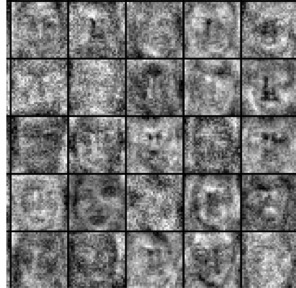
\includegraphics[width=100mm]{img/c6/filter}
 \end{center}
 \caption{実験で学習されたフィルター}
 \label{c6_filter}
\end{figure}
%% !TEX root = thesis.tex
\chapter{Facebookの顔画像認識と深層学習技術}
この章では、深層学習を画像認識の問題に適用した応用例を挙げる。\par
ソーシャルメディアのユーザ属性を推定することは、マーケティングやネット広告の最適化において有益である。ここでは、公開プロフィールの一種であるプロフィール画像に着目する。入力となるプロフィール画像と、推定する目標であるユーザ属性のセットを用いて、深層学習を行わせることで、より精度の高いユーザ属性推定を目指す。

\section{背景}
ソーシャルメディアのユーザプロフィールから、そのユーザの属性を推定するためのアルゴリズムが求められている。\\
マーケティングや、ネット広告の最適化などに応用可能で、ビジネス面において大きな貢献が期待できる。\par
ユーザ属性の推定元としては、名前 / 日記 / ツイートなどのテキストデータ、プロフィールなどの画像、友達関係などが挙げられる。\cite{pennacchiotti2011a-machine}

テキストデータは量が豊富だが、ソーシャルメディアの種類によっては、「友達のみ公開」などの設定がされている。ネット広告を載せる企業の視点から見ると、常に自由にアクセスできるとは限らない。\\

一方プロフィール画像は、ほぼ全てのソーシャルメディアにおいて、全員に公開されている。ネット広告企業からでも、必ずチェックできる。\\

画像からユーザ属性を推定できれば、より多くの場面で、効率の良いマーケティングが可能になる。これはテキストベースの方法にはない、大きなメリットである。\\

しかし、プロフィール画像を元データとした研究はまだメジャーではない。\\
最終的に、ソーシャルメディアのプロフィール画像が与えられれば、ユーザ属性を推定できる状態を目指す。\\
その過程として、今回の領域プロジェクトでは、「Facebook」より「プロフィール顔画像」に限定してのユーザ推定を試みる。\par

\begin{figure}[tbp]
 \begin{center}
  \includegraphics[width=100mm]{img/c7/prof2prop}
 \end{center}
 \caption{ユーザ属性推定の必要性}
 \label{c7_prof2prop}
\end{figure}

公開プロフィールからユーザ属性を推定するというアプローチによる過去の研究としては、Twitterのプロフィールやツイート内容、フォロー関係などから、ユーザ属性を割り出したものがある\cite{pennacchiotti2011a-machine}。この研究では、「スターバックスが好きか」「支持政党は民主党と共和党のどちらか」「どの民族 (ethnicity)に属しているか」といった情報を推定している。\par
なお、この研究においては、プロフィール写真はユーザ属性を推定する参考になりにくいとされている。彼らに拠れば、ソーシャルメディアのユーザーは、必ずしもプロフィール画像にユー
ザ本人の画像を用いるわけではない。むしろ、有名人の画像が使われていて、本人の属性推定においてノイズとなってしまうケースもある。\par
また、別の研究\cite{mislove2011understanding}では、Twitterのデータより、Twitterのユーザ構成の傾向について、基本的なデータを収集している。具体的には、位置情報より居住地の傾向を、first nameから性別の傾向を、last nameから宗教の傾向を割り出している。なお、この研究でもプロフィール画像データは用いられていなかった。\par
H. Andrew Schwartzらは、公開プロフィールという制限こそ課していないが、75000名のユーザ有志より、7000万個の単語や言葉、話題の例を収集して分析にかけ、同時に収集した年齢・性別・性格テストのデータとの相関性を学習させることや、言葉遣いからこれらのユーザ属性を精度良く推測させることに成功した\cite{schwartz2013personality}。彼らは、年代や性格ごとに特徴的な言葉遣いを可視化しており、可視化の結果はウェブサイトにて見ることができる\footnote{\url{http://wwbp.org/}}。

\begin{figure}[tbp]
 \begin{center}
  \includegraphics[width=100mm]{img/c7/pic_sample}
 \end{center}
 \caption{Facebookにおけるプロフィール画像の例}
 \label{c7_pic_sample}
\end{figure}

\section{ソーシャルメディアにおける、プロフィール画像}
図\ref{c7_pic_sample}に、実際にFacebookにて利用されているプロフィール画像の例を挙げる。これはごく一部の例であるが、これらを見るだけでも、以下の障害となりそうな点が考えられる。
\begin{itemize}
\item \textbf{人間が写っているとは限らない。}人気キャラクターやブランドのロゴ、絵画が含まれている。入力データのバリエーションが増えることで、学習が難しくなることが予想される。
\item \textbf{2人以上の人間が映っていることがある。}例えば、カップルの写真やクラスの集合写真がプロフィール画像として使われていたとき、誰がユーザ本人であるかを推定するのは極めて困難だと想像できる。
\item \textbf{本人の画像かどうかわからない。}先述した研究\cite{pennacchiotti2011a-machine}でも述べられている通り、少なくとも画像自体の中に、本人である証拠はない。有名人に関しては、有名人の顔写真のデータベースを別途作成することで対応できる可能性があるが、あまり知られていない他人の写真だった場合、対処は難しい。
\item \textbf{顔が鮮明でないことがある。}例え本人が写っていても、顔の拡大写真ではなく、全身が映されていて、顔がぼやけてしまっていることがある。
\end{itemize}
以上をまとめると、「プロフィール画像=ユーザの顔」という前提が成り立たないという問題点が浮き彫りになる。この前提が成り立たない場合、「画像 = ユーザの顔→ユーザの年齢や性別」という一段階の推論ではなく、「画像→本人か?→本人でなかったら、誰の容姿なのか、またはキャラクターやブランドなのか→その有名人やキャラクターを好むユーザは、どのような年齢や性別が多いか?」という多段階の推論が必要となり、学習難易度が高くなると考えられる。\par
今回は、

\section{提案手法}
図\ref{c7_proposal}は、今回の提案手法を表している。提案手法は、次の3ステップより成る。
\begin{enumerate}
\item \textbf{ソーシャルメディアより、プロフィール画像を得る。}この方法はソーシャルメディア毎に大きく異なるが、各メディアが提供しているAPIや、閲覧者用のウェブページより、様々なユーザのプロフィール画像を取得する。また、このときユーザ属性の教師データを取得できる場合もある。
\item \textbf{プロフィール画像を、ベクトルデータに変換する。}基本的には、画像の各画素値そのものを、入力ベクトルとして使用する。これは、可能な限り取得したままのデータを加工せずに入力することで、素性の採り方自体を学習できる深層学習の特徴を活かせるからである。ただし,対象データによっては,画像の特徴量を付加することで精度が上昇する\cite{ciresan2012multi-column}ことが知られており、工夫の余地もある。
\item \textbf{ベクトルデータから、分類器を使って、ユーザ属性を識別する。}機械学習により、画像のベクトルデータからユーザ属性を推定できるような、クラス識別モデルを取得する。深層学習が応用されるのは、この部分である。
\end{enumerate}


\begin{figure}[tbp]
 \begin{center}
  \includegraphics[width=100mm]{img/c7/proposal}
 \end{center}
 \caption{提案手法}
 \label{c7_proposal}
\end{figure}

\section{問題設定と、実験方法の詳細}
今回の実験では、ソーシャルメディアのプロフィール画像からユーザ属性を推定する例として、Facebookのプロフィール画像のうち、人間の顔画像を1つだけ含んでいるものを対象として、ユーザの性別を推定出来るかどうか、学習を行わせた。以下に、実験方法の詳細を記す。
\subsection{画像の取得と加工}
Facebookの公開APIを用いて、サイズ200x200(px)のプロフィール画像を11028件取得した。画像と同時に、ユーザの性別データも収集した。\par
取得した画像からは、条件に合わないものを除外すると同時に、顔の特徴が失われない範囲で、学習速度を上げるための前処理を施した。まず、各画像をRGBカラーからグレースケールに変換した。次に、人間の顔画像がちょうど1人分入っているかどうか、判定を行った。これには画像処理ライブラリのOpenCVに含まれている、顔画像識別のプログラム\footnote{\url{http://docs.opencv.org/trunk/modules/objdetect/doc/cascade_classification.html}}を用いた。識別器には、LBP Cascade法\cite{liao2007learning}を使った。判別の結果、サイズ20x20[px]以上で正面を向いた1人分の顔画像が検出できた場合のみ、その画像を使用した(図\ref{c7_pic_sample})。さらに、検出した顔領域が中心で一定のサイズを占めるように、画像を切り抜き、30x30[px]に解像度を落とした。また、より画像の特徴がわかりやすくなって学習が進むよう、色調を平均化補正し、コントラストが際立つようにした。\par
以上の行程により、男性2180件、女性1566件、計3746件の画像データ及び、対応する性別のデータが集まった。
\subsection{ベクトルデータへの変換}
平面的な広がりを持つ画像データから、画素値[0.0-1.0)を要素とする900次元のベクトルデータへの変換を施した。画像の各画素と、ベクトルの順番の関係は、図\ref{c7_conv}のようになっており、この図における画素の番号と、ベクトルの要素番号が対応している。
\subsection{ユーザの分類}
入力がここまでの変換で得たベクトルデータ、出力がユーザの性別の、クラス分類問題として考える。
分類器に学習を行わせ、ユーザを精度よく分類することを目指す。学習モデルとしては、深層ニューラルネットワークの一種である積層雑音除去自己符号器(以下SDA)と、従来手法としてのサポートベクターマシン(以下SVM)の2つを用いた。\par
SDAの実装には,ウェブサイトDeep Learning Tutorial\footnote{\url{http://www.deeplearning.net/tutorial}}にて提供されているものを用いた。corruption rateは30\%とした。また、SVMの実装には、専用ライブラリのLIBSVM\footnote{\url{http://www.csie.ntu.edu.tw/~cjlin/LIBSVM/}}を用いた。
\par

\begin{figure}[tbp]
 \begin{center}
  \includegraphics[width=80mm]{img/c7/expr}
 \end{center}
 \caption{今回の実験の模式図}
 \label{c7_expr}
\end{figure}

\begin{figure}[tbp]
 \begin{center}
  \includegraphics[width=80mm]{img/c7/conv}
 \end{center}
 \caption{実験で使った、画像から入力ベクトルへの変換方法}
 \label{c7_conv}
\end{figure}

\begin{figure}[tbp]
 \begin{center}
  \includegraphics[width=80mm]{img/c7/pic_judge}
 \end{center}
 \caption{プロフィール画像からの顔画像抽出方法}
 \label{c7_pic_judge}
\end{figure}

\section{結果}
分類精度は、表\ref{c7_fb_result}の通りとなった。深層学習のSDAの方が、少し精度が低い結果となってしまった。\par
\begin{table}[tbp]
 \begin{center}
  \includegraphics[width=60mm]{img/c7/fb_result}
 \end{center}
 \caption{Facebook顔画像の分類結果}
 \label{c7_fb_result}
\end{table}
なお、図\ref{c7_フィルタ}に、今回の実験でSDAが学習した、1レイヤー目のフィルターを示す。SDAは精度こそ僅かに劣っているものの、今回の方法でも顔を学習すること自体には成功していることがわかる。

\begin{figure}[tbp]
 \begin{center}
  \includegraphics[width=100mm]{img/c7/フィルタ}
 \end{center}
 \caption{実験で学習されたフィルター}
 \label{c7_フィルタ}
\end{figure}

\section{考察}
\subsection{全体の結果のまとめ}
この章の実験では、ソーシャルメディアのユーザ属性推定において、プロフィール画像からの推定手法を模索した。実験の結果、SDA、SVM共に、Facebookのユーザプロフィールにて1人分の顔画像が使われているという条件ならば、ある程度ユーザの性別を識別できることがわかった。\par
\subsection{SDAにて良い精度が出なかった理由の考察}
識別自体にはある程度成功したとはいえ、本来画像認識や多段階の推論で効果を発揮すると思われる深層学習を使用したにも関わらず、従来から用いられている単純なSVMによる精度を上回ることが出来なかった。この理由はわかっていないが、考えられることとして、まず実験で用意したデータ数の不足や偏りが考えられる。例えば、深層学習全般が大きな成果を挙げているMNISTのデータセットには、全体で70000のデータが用意されている。また、CIFAR10でも60000件のデータが利用可能である。比べて、今回用意できたデータは3746件のみであり、男性と女性のデータ数には1.3倍ほどの開きがあった。このデータの不足と偏りが、学習傾向に歪みを与えてしまった可能性がある。\par
また、隠れレイヤー数、レイヤー内ユニット数など、学習モデルを形成する様々なハイパーパラメータの調整を行うことで、学習制度を向上させることができる可能性がある。SVMの場合、grid searchと呼ばれる方法によってパラメータを調整している。しかし、この方法はハイパーパラメータが増加するにつれて指数関数的にかかる時間が増大してしまう。パラメータが1〜3個程度で済むSVMでは有効な方法だが、パラメータ数が非常に多いSDAや他の深層学習の方法では、現実的ではない。ハイパーパラメータを自動的に調整する方法が必要である。\par
ハイパーパラメータを調整する方法としては、\cite{bengio2012practical}にて、Grid Searchによってしらみつぶしに探すよりも、Random Searchを用いた方が効率が良いと述べられており、今後実験を行う際には参考にしようと思う。また、実験用ビルドシステムを併用することも効果的だと思われる\footnote{\url{https://github.com/pfi/maf}}。

\subsection{今後の発展について}
今回の実験では、まず最も確実性の高いところから検証するということで、単体の顔プロフィール画像のみを識別のターゲットとした。しかし、キャラクターやブランドロゴなどの非実写アイコンや、人間の横顔、複数人が映った画像からでもユーザ属性が推定できれば、より応用での確実性が増す。性別だけでなく、ユーザの好みや交友関係の傾向も推測できれば、これも貴重な情報となる。人間の行動や思考は、テキストだけでなく、ファッションや交友関係など非言語的な特徴にも顕れる。こういった情報も学習できるようになれば、システムの利用価値が高くなっていくと思われる。\par
Facebookは、本人画像の使用率が比較的高いコミュニティとして一般に知られている。有名人の画像利用問題が考えられるにも関わらず、ある程度精度良く識別が出来たのも、対象がFacebookだったからということは考えられる。Facebookだけでなく、Twitterなど、本人画像以外がプロフィール画像に使われやすいソーシャルメディアでも、ユーザ属性が推定出来れば、応用が容易になると考えられる。

% !TEX root = thesis.tex
\chapter{おわりに}
\section{研究の成果}
この研究では、深層学習をウェブ工学の問題に適用するにあたって、その特徴である高い精度を落とすことなく、出来るだけ簡便に応用するための方法論とノウハウを調査した。Pylearn2に実装されている、Maxout Networkを用いることで、論文に書かれている精度をほぼ再現することが出来た。また、GPUを使うと大幅な高速化が見込めることがわかった。

\section{今後の課題}
画像分類タスクにおいて有効な方法が、ウェブ工学のデータでも必ず有効かどうかは、未知数な部分がある。例えば、畳み込みネットワークは、2次元の画像データに対しては非常に高い効果を挙げるが、そのまま文章データに応用することは出来ない。Pylearn2で言えば、Datasetクラスを作るだけで識別がうまくいくのか、文章専用のModelを構成する必要があるのか、確かめていく必要がある。\par
また、精度を上げるためには、どのようにハイパーパラメータを調整すれば良いのか、あるいは精度を多少犠牲にしてでも、比較的短い実行時間で良い結果を得たい時、どのような調整を施せばよいのかは、まだわかっておらず、今後の大きな課題の一つである。\par
現在の深層学習が比較的得意とする画像データ処理について、単純な認識タスクで大量の訓練データが用意されている条件ならば、畳み込みレイヤーによる特徴抽出が非常に良い性能を示す。しかし、問題設定を少し変えて、「シンボルを1つだけ見せて、他のシンボルの中から同じものを選ばせる(one-shot classification)」「シンボルを1つだけ見せて、同じシンボルを機械と人間に書かせ、どちらが上手く出来るか競う(one-shot generation)」といった、データ数が非常に少ない条件下では、まだ人間が手間をかけて作った素性を使った方が性能が高いことがある\cite{lake2013one}。画像をただ認識するだけでなく、良い素性の作り方を少ないデータから学習できるようになれば、繰り返し回数を減らし学習時間を短縮することにもつながり、応用の幅が広がると思われる。\par
深層学習を試す上で、大きなネックとなるのが、CUDAを用いたGPU専用のソースコードの存在である。GPUを搭載していなかったり、使えるメモリが少ない状況下でも、深層学習のコードを効率良く動かすことが出来れば、深層学習の利便性はますます増加するだろう。\par
現在の深層学習では、画像のフィルタで何が学習されているのかを、部分的に可視化することはできる。しかし、文書解析において、どのような表現を学習したのかを、人間に理解できる形でみることは難しい。言い換えれば、学習によって、分類器がどこに注目するようになったのか、文構造や、感情、文体などに対応するニューロンが存在しているのか、といった情報が、人間に理解できる形になっていない。この部分をどうやって可視化して、人間に理解できる状態にするか、そこからどのような知見を得られるのか、あるいはそもそも人間には理解出来る知識として取り出せるのかどうか、といったことを調べることにより、表現学習としての深層学習の側面を、さらに活かすことができると思われる。例えば、深層学習にょって学習された、データの着目点や抽象化のポイントを、人間が真似することによって、人間の方が機械から知識を習得し、さらに発展させることも考えられる。

%
% !TEX root = thesis.tex
\chapter*{謝辞}
\addcontentsline{toc}{chapter}{謝辞}
本研究の執筆にあたり、指導教官である東京大学大学院工学系研究科技術経営戦略学専攻・総合研究機構・知の構造化センター准教授である松尾豊先生は、研究テーマの方向性を決める初期段階から何度も相談に乗って頂き、ご多忙の中私の曖昧な質問にも快くアドバイスを返して下さいました。また、調査・実験段階でも私が研究の方向性を見失わないよう助言をして下さった他、執筆段階では論文の書き方の基本的な心構えから教えてくださり、私の拙い草稿に何度も目を通して、修正のコメントをして下さいました。\par
東京大学知の構造化センター特任講師の中山浩太郎先生は、深層学習の実装段階において、ハードウェアとソフトウェア両面の多彩な知識によって、深層学習の研究を支えてくださり、また様々な補助ライブラリを提供して下さいました。東京大学情報理工学系研究科創造情報学専攻講師の中山英樹先生からは、画像認識研究の基本的なポイントについて、貴重な示唆を頂きました。\par
東京大学松尾研究室博士課程の大澤さんは、研究生活の全行程に渡って、何をすれば良いのかゼロから手取り足取り教えてくださいました。特に、執筆段階では、私がどのような初歩的な質問をしても、懇切丁寧に教えて下さり、執筆の大きな助けを頂きました。同研究室博士課程の榊さん、沼さん、関さんにも、研究の基本やテーマの方向性、スケジュールの考え方や執筆ソフトの扱いなどについて、様々なことを教えて頂きました。同研究室修士課程の飯塚さんや、同研究員の那須野さんには、ご自身も研究でお忙しい中、度重なる私のサーバ関連の報告に対して、長時間の対応をして下さり、非常に助かりました。同研究室学部4年生の川上さん、キムさん、安野さんには、長い卒業論文執筆期間の中で何度も励まされ、また時には切磋琢磨する相手としての緊張感をももたらして下さいました。他研究室のメンバーの方々にも、研究会を始めとして様々な場面で助言や励ましの言葉を頂きました。\par
本研究は、様々な方の協力が無くては完成し得ないものでした。ここにお礼を申し上げます。ありがとうございました。

\begin{flushright}
東京大学工学部システム創成学科 \\
知能社会システムコース\\
松尾研究室 4年 黒滝 紘生\\
平成26年2月6日\\
\end{flushright}
%
\bibliographystyle{jplain_mod}
\bibliography{research}
%
\end{document}
